%%%%%%%%%%%%%%%%%%%%%%%%%%%%%%%%%%%%%%%%%%%%%%%%%%%%%%%%%%%%%%%%%%%%
%%%%%%%%%%%%%%%%%%%%%%%%%%%%%%%%%%%%%%%%%%%%%%%%%%%%%%%%%%%%%%%%%%%%
%%                                                                %%
%% Esimerkki opinnäytteen tekemisestä LaTeX:lla 20130926          %%
%% Alkuperäinen versio Luis Costa,  muutokset Perttu Puska        %%
%%                                                                %%
%% Tähän esimerkkiin kuuluu tiedostot                             %%
%%               opinnaytepohja.tex (versio 1.7)                  %%
%%               aaltothesis.sty (versio 1.7)                     %%
%%               kuva1.eps                                        %%
%%               kuva2.eps                                        %%
%%                                                                %%
%%                                                                %%
%% Kääntäminen                                                    %%
%% latex:                                                         %%
%%             $ latex opinnaytepohja                             %%
%%             $ latex opinnaytepohja                             %%
%%                                                                %%
%%   Tuloksena on tiedosto opinnayte.dvi, joka                    %%
%%   muutetaan ps-muotoon seuraavasti                             %%
%%                                                                %%
%%             $ dvips opinnaytepohja -o                          %%
%%                                                                %%
%% Selittävät kommentit on tässä esimerkissä varustettu           %%
%% %%-merkeillä ja muutokset, joita käyttäjä voi tehdä,           %%
%% on varustettu %-merkeillä                                      %%
%%                                                                %%
%%%%%%%%%%%%%%%%%%%%%%%%%%%%%%%%%%%%%%%%%%%%%%%%%%%%%%%%%%%%%%%%%%%%
%%%%%%%%%%%%%%%%%%%%%%%%%%%%%%%%%%%%%%%%%%%%%%%%%%%%%%%%%%%%%%%%%%%%

%% Käytä toinen näistä, jos kirjoitat suomeksi:
%% ensimmäinen, jos käytät pdflatexia (kuvat on oltava pdf-tiedostoina)
%% toinen, jos haluat tuottaa ps-tiedostoa (käytä eps-formaattia kuville).
%%
%% Use one of these you write in Finnish:
%% the 1st when using pdflatex (use pdf figures) or
%% the 2nd when producing a ps file (use eps figures).
\documentclass[finnish,12pt,a4paper,pdftex]{article}
%\documentclass[finnish,12pt,a4paper,dvips]{article}


%% Käytä näitä, jos kirjoitat englanniksi
%%
%% Uncomment one of these if you write in English
%\documentclass[english,12pt,a4paper,pdftex]{article}
%\documentclass[english,12pt,a4paper,dvips]{article}

%% Tämä paketti on pakollinen
%% Valitse korkeakoulusi näistä: arts, biz, chem, elec, eng, sci.
%% Valiste editorisi käyttämä merkkikoodaustapa: utf8, latin1
%%
%% This package is required
%% Choose your school from arts, biz, chem, elec, eng, sci.
%% Choose the character encoding scheme used by your editor: utf8, latin1
\usepackage[sci,utf8]{aaltothesis} % this is the default in aaltothesis.sty
%\usepackage[elec,latin1]{aaltothesis}

%% Jos käytät latex-komentoa käännettäessä (oletusarvo), 
%% kuvat kannattaa tehdä eps-muotoon. Älä käytä ps-muotoisia kuvia!
%% Käytä seuraavaa latex-komennon ja eps-kuvien kanssa 
%%
%% Jos taas käytät pdflatex-komentoa, joka kääntää tekstin suoraan
%% pdf-tiedostoksi, kuvasi on oltava jpg-formaatissa tai pdf-formaatissa.
%%
%% Use this if you run pdflatex and use jpg/pdf-format pictures.
%%
\usepackage{graphicx}

\usepackage[table,xcdraw]{xcolor}

%% Jos et jostain syystä pidä, miten alla oleva hyperref-paketti käyttää
%% fontteja, värejä yms., käytä tämän paketin makroja muuttamaan
%% fonttimäärittelyt. Katso paketin dokumentaatiota. Paketti määrittelee
%% \url-makron, joten ota paketti käyttöön, jos et käytä hyperref-pakettia.
%%
%% Use the macros in this package to change how the hyperref package below 
%% typesets its hypertext -- hyperlink colour, font, etc. See the package
%% documentation. It also defines the \url macro, so use the package when 
%% not using the hyperref package.
%\usepackage{url}

%% Saat pdf-tiedoston viittaukset ja linkit kuntoon seuraavalla paketilla.
%% Paketti toimii erityisen hyvin pdflatexin kanssa. 
%%
%% Use this if you want to get links and nice output with pdflatex
%%
\usepackage[pdfpagemode=None,colorlinks=true,urlcolor=red,%
linkcolor=blue,citecolor=black,pdfstartview=FitH]{hyperref}

\graphicspath{ {images/} }

\usepackage[round]{natbib}
\bibliographystyle{agsm}

%%Vaihdetaan sitaateissa and-sana ja-sanaksi
\AtBeginDocument{\renewcommand{\harvardand}{ja}}

%% Matematiikan fontteja, symboleja ja muotoiluja lisää, näitä tarvitaan usein 
%%
%% Use this if you write hard core mathematics, these are usually needed
\usepackage{amsfonts,amssymb,amsbsy}  

%% Vaakasuunnan mitat, ÄLÄ KOSKE!
\setlength{\hoffset}{-1in}
\setlength{\oddsidemargin}{35mm}
\setlength{\evensidemargin}{25mm}
\setlength{\textwidth}{15cm}
%% Pystysuunnan mitat, ÄLÄ KOSKE!
\setlength{\voffset}{-1in}
\setlength{\headsep}{7mm}
\setlength{\headheight}{1em}
\setlength{\topmargin}{25mm-\headheight-\headsep}
\setlength{\textheight}{23cm}


%% Kaikki mikä paperille tulostuu, on tämän jälkeen
%%
%% Output starts here
\begin{document}

%% Korjaa vastaamaan korkeakouluasi, jos automaattisesti asetettu nimi on 
%% virheellinen 
%%
%% Change the school field to describe your school if the autimatically 
%% set name is wrong
% \university{aalto University}{aalto-Yliopisto}
% \school{School of Science}{Perustieteiden korkeakoulu}

%% Vain kandityölle: Korjaa seuraavat vastaamaan koulutusohjelmaasi
%%
%% Only for B.Sc. thesis: Choose your degree programme. 
%%\degreeprogram{Electronics and electrical engineering}%
%%{Elektroniikka ja sähkötekniikka}
%%

%% Vain DI/M.Sc.- ja lisensiaatintyölle: valitse laitos, 
%% professuuri ja sen professuurikoodi. 
%%
%% Only for M.Sc. and Licentiate thesis: Choose your department,
%% professorship and professorship code. 
%%\department{Department of Radio Science and Technology}%
%%{Radiotieteen ja -tekniikan laitos}
\professorship{ICT Business}{ICT liiketoiminta}
\code{???}
%%

%% Valitse yksi näistä kolmesta
%%
%% Choose one of these:
%\univdegree{BSc}
\univdegree{MSc}
%\univdegree{Lic}

%% Oma nimi
%%
%% Should be self explanatory...
\author{Jaakko Lehtinen}

%% Opinnäytteen otsikko tulee vain tähän. Älä tavuta otsikkoa ja
%% vältä liian pitkää otsikkotekstiä. Jos latex ryhmittelee otsikon
%% huonosti, voit joutua pakottamaan rivinvaihdon \\ kontrollimerkillä.
%% Muista että otsikkoja ei tavuteta! 
%% Jos otsikossa on ja-sana, se ei jää rivin viimeiseksi sanaksi 
%% vaan aloittaa uuden rivin.
%% 
%% Your thesis title. If the title is very long and the latex 
%% does unsatisfactory job of breaking the lines, you will have to
%% break the lines yourself with \\ control character. 
%% Do not hyphenate titles.
\thesistitle{Thesis template}{LISÄÄ NIMI}

\place{Espoo}
%% Kandidaatintyön päivämäärä on sen esityspäivämäärä! 
%% 
%% For B.Sc. thesis use the date when you present your thesis. 
\date{KORJAA: 24.9.2013}

%% Kandidaattiseminaarin vastuuopettaja tai diplomityön valvoja.
%% Huomaa tittelissä "\" -merkki pisteen jälkeen, 
%% ennen välilyöntiä ja seuraavaa merkkijonoa. 
%% Näin tehdään, koska kyseessä ei ole lauseen loppu, jonka jälkeen tulee 
%% hieman pidempi väli vaan halutaan tavallinen väli.
%%
%% B.Sc. or M.Sc. thesis supervisor 
%% Note the "\" after the comma. This forces the following space to be 
%% a normal interword space, not the space that starts a new sentence. 
\supervisor{Prof.\ Martti Mäntylä}{Prof.\ Martti Mäntylä}

%% Kandidaatintyön ohjaaja(t) tai diplomityön ohjaaja(t)
%% 
%% B.Sc. or M.Sc. thesis advisors(s). 
%%
%% Note that there has been a change in the official EN translation
%% of the Finnish title ``ohjaaja'' which in the previous version (1.5) 
%% of this document was called ``instructor''. The recommended
%% translation is now ``advisor''.  
%% However, the LaTeX internal variable remains \instructor
%% as there is little point to change the variable name. 
%%
%\instructor{Prof. Pirjo Professori}{Prof. Pirjo Professori}
%\instructor{D.Sc.\ (Tech.) Olli Ohjaaja}{TkT Olli Ohjaaja}
\instructor{M.Sc.\ (Tech.) Tapio Jakola}{DI Tapio Jakola}

%% Aaltologo: syntaksi:
%% \uselogo{aaltoRed|aaltoBlue|aaltoYellow|aaltoGray|aaltoGrayScale}{?|!|''}
%% Logon kieli on sama kuin dokumentin kieli
%%
%% Aalto logo: syntax:
% \uselogo{aaltoRed|aaltoBlue|aaltoYellow|aaltoGray|aaltoGrayScale}{?|!|''}
%% Logo language is set to be the same as the document language.
\uselogo{aaltoRed}{''}

%% Tehdään kansilehti
%%
%% Create the coverpage
\makecoverpage


%% Suomenkielinen tiivistelmä
%% 
%% Finnish abstract
%%
%% Tiivistelmän avainsanat
\keywords{Avainsanoiksi valitaan kirjoituksen sisältöä keskeisesti kuvaavia
käsitteitä}
%% Tiivistelmän tekstiosa
\begin{abstractpage}[finnish]
  Tiivistelmässä on lyhyt selvitys (noin 100 sanaa)
  kirjoituksen tärkeimmästä sisällöstä: mitä ja miten on tutkittu,
  sekä mitä tuloksia on saatu. 
  Tiivistelmässä on lyhyt selvitys (noin 100 sanaa)
  kirjoituksen tärkeimmästä sisällöstä: mitä ja miten on tutkittu,
  sekä mitä tuloksia on saatu. 

  Tiivistelmässä on lyhyt selvitys (noin 100 sanaa)
  kirjoituksen tärkeimmästä sisällöstä: mitä ja miten on tutkittu,
  sekä mitä tuloksia on saatu. 
  Tiivistelmässä on lyhyt selvitys (noin 100 sanaa)
  kirjoituksen tärkeimmästä sisällöstä: mitä ja miten on tutkittu,
  sekä mitä tuloksia on saatu. 
  Tiivistelmässä on lyhyt selvitys (noin 100 sanaa)
  kirjoituksen tärkeimmästä sisällöstä: mitä ja miten on tutkittu,
  sekä mitä tuloksia on saatu. 
\end{abstractpage}

%% Pakotetaan uusi sivu varmuuden vuoksi, jotta 
%% mahdollinen suomenkielinen ja englanninkielinen tiivistelmä
%% eivät tule vahingossakaan samalle sivulle
%%
%% Force new page so that English abstract starts from a new page
\newpage
%
%% English abstract, uncomment if you need one. 
%% 
%% Abstract keywords
\keywords{}
%% Abstract text
\begin{abstractpage}[english]
 Your abstract in English. Try to keep the abstract short, approximately 
 100 words should be enough. Abstract explains your research topic, 
 the methods you have used, and the results you obtained.  
\end{abstractpage}
%% Note that 
%% if you are writting your master's thesis in English place the English
%% abstract first followed by the possible Finnish abstract

%% Esipuhe 
%%
%% Preface
\mysection{Esipuhe}
%\mysection{Preface}
Lisää tähän esipuhe.\\

\vspace{5cm}
Otaniemi, 24.9.2013

\vspace{5mm}
{\hfill T T.\ A.\ Teekkari \hspace{1cm}}

%% Pakotetaan varmuuden vuoksi esipuheen jälkeinen osa
%% alkamaan uudelta sivulta
%%
%% Force new page after preface
\newpage


%% Sisällysluettelo
%% 
%% Table of contents. 
\thesistableofcontents


%% Symbolit ja lyhenteet
%%
%% Symbols and abbreviations
\mysection{Käsitteet}
%\mysection{Symbols and abbreviations}




%% Sivulaskurin viilausta opinnäytteen vaatimusten mukaan:
%% Aloitetaan sivunumerointi arabialaisilla numeroilla (ja jätetään
%% leipätekstin ensimmäinen sivu tyhjäksi, 
%% ks. alla \thispagestyle{empty}).
%% Pakotetaan lisäksi ensimmäinen varsinainen tekstisivu alkamaan 
%% uudelta sivulta clearpage-komennolla. 
%% clearpage on melkein samanlainen kuin newpage, mutta 
%% flushaa myös LaTeX:n floatit 
%% 
%% Corrects the page numbering, there is no need to change these
\cleardoublepage
\storeinipagenumber
\pagenumbering{arabic}
\setcounter{page}{1}


%% Leipäteksti alkaa
%%
%% Text body begins. Note that since the text body
%% is mostly in Finnish the majority of comments are
%% also in Finnish after this point. There is no point in explaining
%% Finnish-language specific thesis conventions in English.
\section{Johdanto}
%\section{Introduction}

%% Ensimmäinen sivu tyhjäksi
%% 
%% Leave first page empty
\thispagestyle{empty}

(Tarvitsee vielä paljon hiomista ja rikastamista muista lähteistä.)

Yrityksen tulee etsiä tapoja säästää resursseja ja mahdollistaa itsepalvelu sen asiakkaille kellonajasta riippumatta, ja nämä tavoitteet ovat parhaiten saavutettavissa IT-palvelujen ja prosessessien automatisoinnilla \citep{lamoureux}. Yritykset aloittivat mekaanisen automatisoinnin jo 1950-luvulla, ja jokainen teknologinen kehitysaskel sen jälkeen on mahdollistanut yhä monimutkaisempien toimintojen automatisoinnin yrityksen toiminnassa. 

Automaatio käsitteenä sai merkityksensä autoteollisuuden tuotantolinjoilta, ja tietotekniikan yleistymisen jälkeen 1970-ja 1980-luvulla yritykset oppivat hyödyntämään automaatiota myös sisäisissä, laskentaa vaativissa prosesseissa, kuten taloushallinnossa. Internetin yleistymisen myötä 1990-2000-luvuilla teknologian kehitys on mahdollistanut liiketoimintaprosessien automatisoinnin. Koko tilaus- ja toimitusketju ja useat tuotteet ja palvelut muuttuivat digitaalisiksi. Automaatiossa ei ole siis pelkästään kysymys ihmistyön antamisesta tietokoneelle, vaan myös sen tekemisestä mikä ei aikaisemmin ollut mahdollista \citep{groover}.

Digitalisaatiosta on puhuttu jo vuosia, ja toistaiseksi se on tarkoittanut sosiaalista mediaa, mobilisaatiota, big data-analytiikkaa ja pilviteknologioiden kehitystä. Digitalisaation seuraavassa vaiheessa on kysymys ohjelmistorobotiikan ja älykkään automaation hyödyntämisestä liiketoiminnan prosesseissa. Voidaan ajatella, että seuraavan ajanjakson aikana teknologia saa aisteja, jotka olivat aikaisemmin vain ihmisen yksinoikeus \citep{groover}.

Teknologisten kehitysaskelten myötä itse teknologia muuttuu kompleksimmaksi ymmärtää, mutta niiden sovelluskohteet monipuolistuvat. Yritysten välisessä kilpailussa kyky hyödyntää uutta teknologiaa ketterästi avaa pienillekin toimijoille ovet kilpailussa jättejä vastaan. Hyvä esimerkki tästä on verkkokaupan kasvu kymmenen viime vuoden aikana. Kuluttajat ovat tottuneet saamaan haluamansa palvelut käyttöönsä yhdellä painalluksella. Sama ilmiö leviää yritysten liiketoimintaan. Odotetaan yhä isompien ja monimutkaisempien palveluiden olevan mahdollisia ottaa käyttöön hetkessä. Tämä tarjoaa pienemmille toimijoille mahdollisuuksia disruptioida markkinoita yksinkertaisella kustannustehokkaalla lähestymistavalla. Teknologinen kehitys tuo yhä monipuolisempia mahdollisuuksia kenelle tahansa luoda jotain joka ei aikaisemmin ollut mahdollista. \citep{lamoureux}

Suuryrityksillä onkin yhä enemmän paineita automatisoida prosessejaan ja investoitava uuteen teknologiaan. Puhutaan transformaatiosta, jossa olemassaolevia tietojärjestelmien määrää vähennetään, toimintoja yksinkertaistetaan,  legacy-järjestelmistä yritetään päästä eroon ja pyritään muuttamaan toimintamalli ketteräksi. Onneksi uudet teknologiat mahdollistavat tämän. Ei ole tarvetta yrittää toimia kuin start up-yritys, on tärkeämpää ymmärtää yritykselle relevantteja teknologioita ja niiden liiketoimintahyötyjä omassa kontekstissa. \citep{lamoureux}

Operaattorin näkökulmasta ilmassa on mahdollisuuksia ja uhkia. McKinseyn tekemän raportin mukaan operaattorit ovat suuressa vaarassa kärsiä disruptiosta markkinoilla. Viiden viime vuoden aikana liikevaihto alalla on ollut hitaasti laskemassa kovan hintakilpailun vuoksi, ja silti investointeja on tehtävä. Data vie koko ajan tilaa perinteisiltä tuottavilta puhe- ja viestintäpalveluilta. Operaattorit ovat vaarassa jäädä tietoliikenneyhteyksien toimittajan rooliin. Onneksi mahdollisuudetkin ovat suuret liiketoiminnan prosessien ja tarjoomien uudistuessa. Raportin mukaan yksi mahdollisuus on kehittää palveluita strategisten kumppaneiden kanssa tavalla, jossa tuotannon ja toimituksen kustannukset ovat minimoitu automatisoinnilla ja digitaalisen asiakaskokemuksen luomisella itsepalvelukanavien kautta.\citep{mckinseytele}

(Tähän parempi aasinsilta)

Asiakaspalveluratkaisujen (contact center) tarjoaminen yritysasiakkaille on ollut operaattoreiden luontaista liiketoimintaa ydinliiketoiminnan ohella. Asiakaspalvelujärjestelmät tarkoittavat yrityksen asiakkaiden yhteydenottojen käsittelemistä yhden järjestelmän kautta kanavasta riippumatta.

Operaattorit ovat olleet vahvoilla tässä liiketoiminnassa puhelinverkkojensa ansiosta. Teknologian kehittymisen myötä puhelinkanavan rinnalle on tullut muita sähköisiä kanavia, ja kanavien määrä kasvaa koko ajan sen mukaan miten asiakkaat haluavat asioida yrityksen kanssa. Kanavasta riippumatta asiakaspalvelujärjestelmän tulisi tarjota asiakaspalvelua tarjoavalle työntekijälle yksi näkymä asiakkaan tietoihin. Yrityksen järjestelmissä on erilaista tietoa asiakkaasta, joka olisi saatava helpoksi näkymäksi yrityksen työntekijälle. Asiakaspalvelujärjestelmä siis integroituu moneen eri järjestelmään ja kanavaan. Tarpeet eri integraatioille kasvavat koko ajan, koska yritykset haluavat tarjota hyvää asiakaskokemusta. Hyvään asiakaskokemukseen vaaditaan paljon tietoa eri järjestelmistä saatavilla helposti ymmärrettävässä muodossa. Asiakaspalvelujärjestelmien kehittäminen on kallista ohjelmistokehitystä, joten operaattorin on ollut helpompi tarjota valitun kumppanin tuotetta asiakkaille ja keskittyä ydinosaamiseensa, eli yhteyksien rakentamiseen asiakastoimituksissa, ja jättää itse järjestelmän kehitys kumppanille. 

Järjestelmiä tarjoavat myös muut kuin operaattorit, ja heidän kilpailuvalttinsa on ollut kustannustehokas tapa toimittaa järjestelmä, asiakaskokemus ja alhaisempi hinta. Itse puhelinkanavan merkityksen vähentyminen tarkoittaa operaattorin ainoan kilpailivaltin merkityksen vähenemistä. Näyttää siis siltä, että operaattorin asemaa asiakaspalvelujärjestelmä-markkinalla disruptoidaan. 

Tässä työssä keskitytään tarkastelemaan
Telia Finland Oyj:n asiakaspalvelujärjestelmää Kontakti L, jolle on asetettu tavoitteeksi automaattinen asiakasprosessi (tilauksen, toimituksen ja laskutuksen osalta), itsepalvelun lisääminen ja kustannustehokkuus. Kyseisellä tuotealueella ei ole aikaisemmin onnistuttu luomaan automaattista asiakasprosessia nykyisissä olosuhteissa. Tarvitaan siis selvitys siitä miten olosuhteiden tulisi muuttua automaattista asiakasprosessia varten.

\subsection{Tutkimuskysymys ja alakysymykset}

Pääkysymys: Tulee varmaankin muuttaa.
Miten asiakasprosessi tulisi rakentaa, että se vastaisi liiketoiminnan tavoitteisiin, eli nopeampiin toimituksiin, asiakastyytyväisyyden parantumiseen, kustannustehokkuuteen, nopeampiin toimintojen lanseerauksiin, mahdollistaisi experimentation and learning in the market place?
Telian täytyy psytyä rakentamaan näiden tuotteiden prosessiin nopeampi uusien teknologioiden kokeilu kuten uudet kanavat  yms. Niitä pitää saada nopeammin asiakkaille!!! Kuvaat miten paljon muutosvoimia tulossa yms ja sitten mites näihin päästään. Noh DevOps ne tuo. Mites DevOps onnistuu nykytilanteessa ja mitä pitää tehdä että sinn päästään?

Se Sofigaten liiketoimintavalmiushomma. Kuvaa nykytila, ja tavoitetila. Mikä estää matkan tavoiteltilaan? 
Mitkä osat asiakasprosessista on kannattava automatisoida?
Telian digitaalisen vision mukaan, onko 80-prosentin automatisaatioaste mahdollista saavuttaa Kontakti L:n asiakasprosessissa?

Mitkä tekijät rajoittavat asiakasprosessin automatisointia?
Miten Kontakti L:n asiakasprosessin tulisi rakentaa Miten asiakaspalvelujärjestelmän asiakasprosessissa voidaan hyödyntää.
Miten Kontakti L:n asiakasprosessi tulee rakentaa, kun siltä odotetaan toimitusvarmuutta, kustannustehokkuutta ja automatisointia.
\begin{itemize}
\item[--]Kysymys 1: Mitkä ovat ne olosuhteet, joissa Kontakti L- asiakaspalvelujärjestelmän asiakasprosessi voidaan automatisoida?
\item[--]Vastaus 1: Kuvaus automatisoidusta asiakasprosessista ja sen vaatimista olosuhteista.
\end{itemize}

Alakysymykset:
\begin{itemize}
\item[--]Kysymys 2: Mitkä ovat ne edellytykset joiden perusteella Kontakti L- asiakaspalvelujärjestelmä on kannattava tarjota digitaalisen itsepalvelukanavan kautta?
\item[--]Vastaus 2: Edellytykset digitaalisen itsepalvelukanavan hyödyntämiselle.
\item[--]Kysymys 3: Missä kohdin automatisoitua asiakasprosessia olisi järkevä hyödyntää robotiikkaa tai älykästä automaatiota?
\item[--]Vastaus 3: Asiakasprosessin vaiheet, joissa robotiikan tai älykkään automaation käyttö on perusteltua.

Todenna komponenteista päättävän henkilön tai materiaalin avulla tukeeko laatutavoite Kontakti L:n asiakasprosessin automatisoimista. 

1. Nykyisten toimintamallien kyky tuottaa tavoitteen mukaisia prosesseja. 
2. Organisaation tarjoamat työkalut ja tuki automatisoinnin rakentamiselle.
3. Olemassa olevien ODI-prosessin komponenttien tuki automatisoinnille

Nykyisissä toimintamalleissa oleva kyky suorittaa tavoitteen mukaisia tehtäviä?
Miten rationaalisesti työprosessissa toimitaan?

Haastattele Jonasta komponenteista, onko tunnistettu teknologia joka johtaa haluttuun lopputulemaan?
Eli jokaisen komponentin osalta tai aliprosessin joka on ODI-prosessin osa, mikä sen osa-alueen liiketoiminnan tavoite on? Onko tunnistettu digitaalinen teknogia joka johtaa tavoitteisiin ja onko ne tavoitteet linjassa Kontakti L-tuotteen kanssa? Tukeeko se tavoitetila automaation lisäämistä Kontakti L:n näkökulmasta
What is the throughput of planned work leading to the goals? 

1. Käsillä olevat komponentit (Zylinc&sisäiset järjestelmät) - miten pitkälle ne tukevat automatisointia, 
minkälaisen automaation ne mahdollistavat?
2. Organisaation tarjoama tuki ja toimintamallit tavoitteen mukaisten prosessien rakentamiseen
automatisoinnin rakentamiselle, onko kärsivällisyyttä?
3. Nykyisten toimintamallien kyky tuottaa tavoitteenmukaisia, 
tässä tapauksessa automaattisia prosesseja jotka pienentävät kustannuksia? 

1. Organisaatio antaa tavoitteen automaatiosta luotavaan prosessiin
Mitä tämä tavoite tarkoittaa? Onko se vain toimituksen näkökulmasta? Otetaanko ylläpitovaihetta huomioon

2. MItä komponentteja organisaatio tarjoaa automaation luomiseksi prosessiin? 

3. Tukevatko nämä komponentit tavoitteen mukaista prosessia?

\end{itemize}
\subsection{Työn rakenne}
Taustatieto kappaleessa kerron yleisesti asiakasprosessista ja mitä sen automatisoinnilla voidaan saavuttaa. Kappaleessa tuodaan myös esille automaation tämän hetken trendejä. Kappale määrittää työn keskeisen konseptin.

Asiakaspalvelujärjestelmät-kappeleessa kuvataan tarkemmin minkälaisestä järjestelmästä on kysymys, eli kuvataan liiketoiminnan ongelma, jonka järjestelmä ratkaisee eri kokoisissa yrityksissä. Kappaleessa tuodaan myös esille minkälaisia järjestelmät ovat luonteeltaan ja minkälaisia tulevaisuuden trendejä on nähtävissä.

Digitaalinen visio-kappaleessa keskitytään antamaan kuva siitä minkälaisia haasteita digitalisaatio ja automatisaatio tuottavat operaattorille, ja miten näitä haasteita on alettu ratkaisemaan.

Yhteenvedossa tuodaan kappaleiden aiheet yhteen ja perustellaan miksi on olennaista tarkastella asiakasjärjestelmän asiakasprosessin automatisointia juuri Telialla.

\subsection{Tutkimuksen rajaus}

Tämä case study tutkii sitä miten prosessin omistajan näkökulmasta (tuotekehitys) tulisi myötä vaikuttaa prosessin automatisointiin kun ollaan Telia nimisellä operaattorilla automatisoimassa Kontkati L nimistä tuotetta joka tulee vendorilta.

%% Opinnäytteessä jokainen osa alkaa uudelta sivulta, joten \clearpage
%%
%% In a thesis, every section starts a new page, hence \clearpage
\clearpage

\section{Taustatieto}



% \section{Background}
\subsection{Asiakasprosessin automatisoiminen ohjelmistotuotannossa}
Kerro tässä kappaleessa mitä asiakasprosessilla tarkoitetaan ohjelmistotuotannossa, ja mitä sen kehittäminen automaattiseksi tarkoittaa. Taustoita myös miksi se haluttaisiin automatisoida. \\
 
Ihminen pyrkii luomaan työkaluja arjen tehtävien helpottamiseksi, ja käytännön kautta ihminen oppii miten työkalua voisi kehittää, kertoo Groover \citeyearpar{groover}. Monimutkaisessa yhä useampia ihmisiä vaativissa toimenpiteissä, kuten ohjelmistotuotannossa, tarvitaan määriteltyjä työkaluja yhteistyölle, eli tapoja toimia yhteisen tavoitteen saavuttamiseksi. \citeauthor{leanit} \citeyearpar{leanit} kertovatkin, että toimintatavat on kannattava määritellä prosessiksi, koska tällöin voidaan standartisoida systemaattinen tapa saavuttaa päämäärä. \citeauthor{leanit} toteavat, että hyötynä prosessien määrittelemisessä ja kuvaamisessa on toiminnan nykytilan havaitseminen, jolloin toimintatapoja voidaan kehittää muuttuvien tarpeiden mukaisesti.

\cite{teollisuustalous} mukaan yritys luo prosesseja muodostaakseen toimintamallit sen tavoitteiden saavuttamiseksi. Heidän mukaansa liiketoiminnan ydinprosessit ovat yrityksen tärkeimpiä arvoa tuottavia prosesseja, ja liiketoimintaprosessissa tavoitellaan tehokasta panoksien ja tuottojen hyötysuhdetta. Haikalan ja Marijärven \citeyearpar{ohjelmistotuotanto} kertovat, että ohjelmistoja ja järjestelmiä tuottavien yritysten liiketoiminnan ydinprosesseihin kuuluu asiakasprosessi, eli prosessi jonka avulla asiakas hankkii ja saa käyttöön haluamansa ohjelmistopalvelun tai -tuotteen. \cite{okaytannot} kuvaavat, että ohjelmistotuotannon prosesseissa on mukana useita ihmisiä yrityksen eri toiminnoista ja yrityksen kumppaniverkostosta, jotka suorittavat tehtäviään orkestroidusti useiden järjestelmien ja työkalujen avulla. Orkestroinnissa korostuvat ohjelmistotuotannon hyväksi havaitut menetelmät ja muut kontekstiin liittyvä prosessit.
 
Se mikä on sopiva tapa ja tarkkuus määrittää prosessi vaihtelee tapauskohtaisesti ja on riippuvainen sovelluskohteesta, \cite{ohjelmistotuotanto} kertovat. Heidän mukaansa liian korkealla tasolla kuvattu prosessi ei välttämättä ohjaa tekemistä tarpeeksi laatutavoitetta kohden, ja liian tarkasti määritetty prosessi ohjaa tekemistä liikaa, jolloin toimintamalleja on työläs muuttaa liiketoiminnan tarpeiden muuttuessa. Haikalan ja Marijärven mukaan sopivan prosessin rakentaminen ohjelmistotuotannossa on aina kompromissi, ja siksi sopiva lähestymistapa on rakentaa mahdollisimman kevyt hallittavissa oleva prosessi. Olennaista heidän mukaansa on prosessille selkeästi määritetty tavoite, jonka saavuttamista on mahdollista seurata prosessin aikana ja jälkeen. 

Lamourexin \citeyearpar{lamoureux} mukaan digitaalisten teknologioiden jatkuva kehitys nopeuttaa innovaatioiden sykliä, jolloin liiketoiminnan tarpeet muuttuvat useammin. Prosessien, jotka vastaavat tarpeen täyttämisestä, täytyy myös mukautua nopeammin tapahtuviin muutoksiin. \cite{teollisuustalous} mukaan laadun jatkuva kehittäminen yrityksen tuotantoprosesseissa johtaa tehokkaampaan asiakasarvon luomiseen vähentämällä asiakasarvoa tuottamattomia työvaiheita ja parantaa näin työn tuottavuutta. \cite{ohjelmistotuotanto} mukaan ihmistyövoima on keskimäärin suurin kustannustekijä ohjelmistotuotannossa. \cite{teollisuustalous} tuovatkin esiin, että automaation käyttöä perustellaankin usein tuottavuuden ja laadun parantumisella. Automaation avulla tuotteita ja palveluita voidaan kehittää nopeammin ja tehokkaammin.

\subsubsection{Asiakasprosessi on liiketoimintaprosessi}

Kuten \cite{teollisuustalous} mainitsivat, liiketoimintaprosessit ovat yrityksen systemaattiset ja standartoidut työkalut niiden tavoitteiden saavuttamiseksi, jonka vuoksi yritys on olemassa. \cite{ohjelmistotuotanto} kertovat, että yrityksen tavoite on ratkaista sen asiakkailla oleva ongelma ja tuottaa ongelman ratkaisemalla lisäarvoa. Siksi heidän mukaansa onkin luonnollista kutsua ohjelmistotuotannossa liiketoiminnan ydinprosessia asiakasprosessiksi.

\begin{figure}[!h]
    \centering
    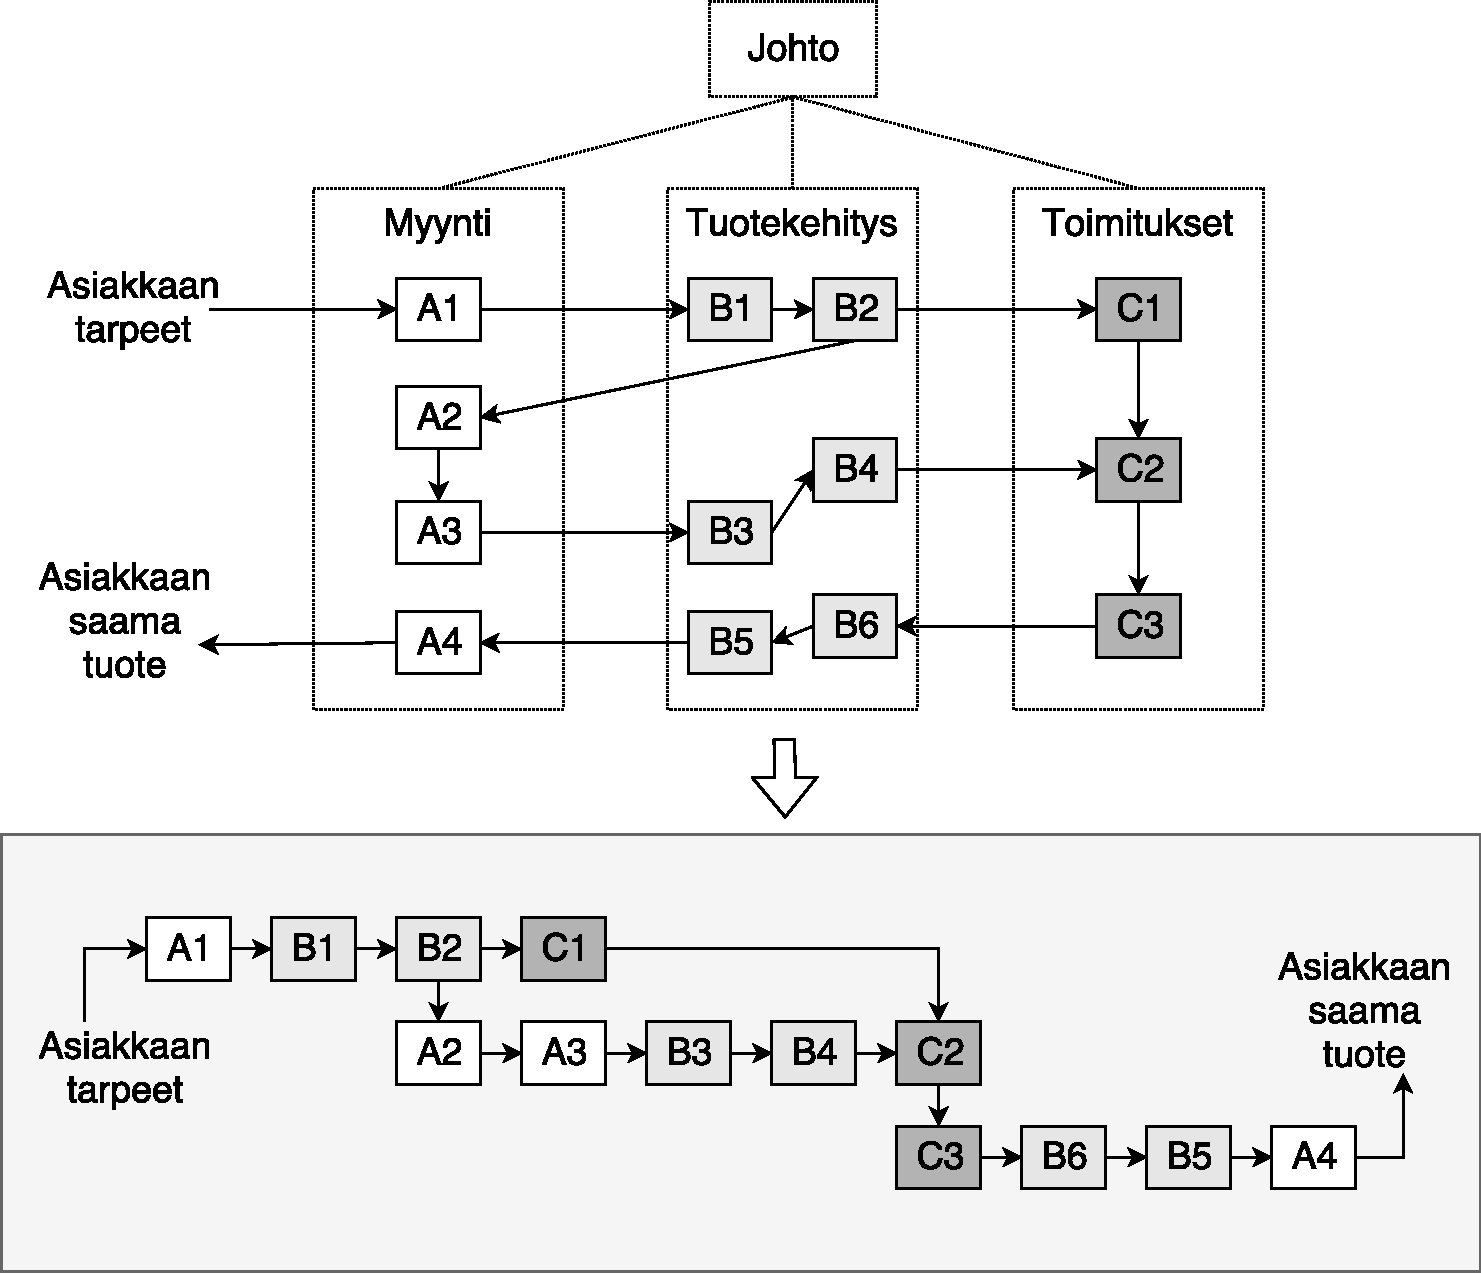
\includegraphics[scale=0.45]{images/Prosessikaavion.pdf}
    \caption{Esimerkki asiakasprosessista. \citep{ohjelmistotuotanto}}
    \label{fig:liikark}
\end{figure}

Kuvassa \ref{fig:liikark} on kuvitteellisen yrityksen asiakasprosessi. Liiketoimintaprosessi synnyttää näin tuotteen asiakkaalle kulkemalla läpi yrityksen eri toimintojen. \cite{ohjelmistotuotanto} tähdentävät, että liiketoiminnan ydinprosessit tuottavat arvoa ulkoiselle asiakkaalle, ja ovat siten tärkeässä roolissa yrityksen tavoitteiden saavuttamisessa. Ydinprosessien apuna on erilaisia tukiprosesseja, joissa asiakas onkin yrityksen sisäinen. Tälläisiä tukiprosesseja on esimerkiksi sisäisten tietojärjestelmien ylläpito tai sisäinen viestintä. \cite{okaytannot} sanovatkin, että liiketoiminnan tukiprosessit eivät välttämättä tuota ydinprosesseihin verrattavaa arvoa, mutta kun ne lakkaavat toimimasta, niillä on huomattavia vaikutuksia yrityksen toimintaan. \citeauthor{okaytannot} huomattavatkin, että liiketoimintaprosessilla on aina asiakas (joko sisäinen tai ulkoinen), joka saavuttaa prosessin avulla haluamansa lopputuloksen. Liiketoimintaprosessi siis ylittää organisaation rajat ja sillä on usein vähän riippuvuutta itse organisaation rakenteeseen.

\cite{leanit} kertovat, että Lean-johtamismallissa liiketoiminnan eri toiminnoista koostuvaa prosessinäkymää kutsutaan arvovirraksi. Heidän mukaansa Lean-johtamismallissa tavoitellaan näkyvää arvotuotannon järjestelmää ja alajärjestelmiä, jolloin huomio voidaan keskittää arvoa tuottamattomien vaiheiden poistamiseen. Arvovirran muodostamassa järjestelmässä muokataan sisään tulevia syötteitä tavoitteen mukaisiksi lopputuloksiksi sen sisältämien prosessien avulla, ja nämä prosessit vaativat, että yritys hankkii ja kuluttaa resursseja. Orzenin ja Paiderin mukaan tyypillisiä yrityksen resursseja ovat esimerkiksi aika, raha, raaka-aineet ja työvoima. He tähdentävät, että se miten yritys päättää järjestää arvoketjun toiminnot ja hallita sitä, määrää tuotannosta aiheutuvat kustannukset ja tuotot. Heidän mukaansa tavoitteena on tehokas arvovirta, joka kuluttaa mahdollisimman vähän resursseja parhaan mahdollisen lopputuloksen aikaansaamiseksi. Orzen ja Paider lisäävät, että toimivan arvovirran laatu on aina mitattavaa ja poikkeamat havaitaan nopeasti prosessin aikana.

Haikalan ja Mikkosen \citeyearpar{okaytannot} mukaan prosessin laadulla ei tarkoiteta ekplisiittisesti hyvää laatua, vaan kontrolloitua laatua valittujen laatutekijöiden perusteella. Kilpailussa markkinoilla korostuu yrityksen valitsemat laatutekijät, koska tuotteiden ja palveluiden laatu rakentuu toimintaprosessien laadusta \citep{ohjelmistotuotanto, teollisuustalous}. \cite{okaytannot} alleviivaavat, että uutta laatutekijää on liki mahdoton lisätä jo rakennettuun ohjelmistotuotteeseen tai -palveluun jälkikäteen, ja sen vuoksi halutut laatutekijät täytyy ottaa huomioon asiakasprosessin kehityksessä. \cite{ohjelmistotuotanto} kertovat, että laatutekijät valitaan mittaamaan liiketoiminnan tavoitteiden toteutumista asiakasprosessin tuloksena. Yrityksen määritelmä laadusta, jolla tavoitteet saavutetaan, antaa suunnan miten arvotuotannon toimintaa johdetaan ja kehitetään. 

Yrityksen valmiuksia parempaan ja tuottavampaan liiketoimintaan voidaan parantaa liiketoimintaprosessien jatkuvalla kehittämisellä \citep{teollisuustalous, leanit, ohjelmistotuotanto}. \citeauthor{ohjelmistotuotanto} kertovat, että prosessin kehittäminen on usein kannattavinta ottamalla pieniä askelia kerrallaan, koska muutoksen läpivieminen saattaa heikentää tuottavuutta hetkellisesti. \cite{devops} kertovat, että prosessissa on kerrallaan vain yksi pullonkaula, jonka täsmällinen kuvaaminen ennen kehitystoimenpiteitä vaatii paljon tarkastelua. Heidän mukaansa prosessin kehittäminen muualla kuin todellisessa pullonkaulassa on prosessin osassa tapahtuva illuusio, eikä siten paranna koko prosessin toimintaa. Haikalan ja Mikkosen \citeyearpar{okaytannot} mukaan prosessien kehittämisessä onnistuminen vaatii ensisijaisesti johdon sitoutumista tukea muutosta, eli käytönnössä aikaa ja resursseja ottaa uusi prosessi käyttöön.

\cite{teollisuustalous} tuovat esiin, että prosessien kehittämisen edellytyksenä on prosessikulttuurin olemassaolo, jolloin voidaan olettaa toiminnan perustuvan prosessien käyttöön, mittaamiseen ja niiden avulla johtamiseen. He toteavat, että ilman prosessikulttuuria olisikin keskityttävä prosessikulttuurin luomiseen riittävissä määrin, koska vain paperilla olevia prosesseja on turha kehittää, koska niillä ei ole yhteyttä todellisiin toimintamalleihin.

\cite{leanit} mukaan liiketoimintaprosessien kehittämisen lähtökohtana on ymmärrys nykytilasta, tavoitetilasta ja näiden kahden tilan erojen tunnistamisesta. Kun näiden kahden tilan väliset erottavat tekijät on tunnistettu, pystytään priorisoimaan kehitystä vaativat osa-alueet. Orzen ja Paider kuvaavat, että riittävä ymmärrys nykytilasta tarkoittaa arvoa tuottavien toimintojen tunnistamistamista, jolloin nähdään missä kohtaa prosessissa on tarpeettomia työvaiheita, joista on hankkiuduttava eroon tai automatisoitava. Ymmärrys tavoitetilasta on heidän mukaansa kuvaus uusista liiketoimintavalmiuksista tai laatuvaatimuksista, joiden perusteella määritetään  toiminnot, jotka tuovat tavoitteen vaatiman arvon. 

\cite{leanit} jatkavat, että liiketoimintaprosessien tarkoituksena liiketoimintaprosessien kehittämisessä joko vähentää resurssien käyttöä ja eliminoida tarpeettomia työvaiheita saman lopputuloksen saavuttamiseksi, tai onnistua löytämään uusia tapoja tuottaa asiakkaalle arvoa prosessin avulla. He lisäävät, että digitaalisten palveluiden myötä avainasemassa on uusien palvelukonseptien kehittäminen ulkoisten sidosryhmien tarpeiden mukaan, jolloin sisäisten ja ulkoisten liiketoimintaprosessien oletetaan taipuvan nopeampiin muutoksen sykleihin.

\cite{teollisuustalous} mukaan suurin este prosessien kehittämiselle on usein heikko ymmärrys nykytilasta, jolloin ei toivotulla tavalla toimivan prosessin laatupoikkeamat havaitaan liian kaukana niiden alkuperäisestä aiheuttajasta. \cite{ohjelmistotuotanto} mukaan ymmärrys prosessin nykytilasta on helppo saavuttaa silloin kun prosessin aktiviteetit ovat selkeästi näkyvillä, ja jokaisella toiminnolla on laatua mittaava komponentti. Heidän mukaansa tällöin prosessin tavoitteen toteutumista voidaan seurata prosessin eri vaiheissa, ja laatupoikkeamien aiheuttaja havaitaan nopeasti. Prosessin omistaja, joka vastaa prosessin kehittämisestä, voi näin kohdistaa kehitystoimenpiteet laatupoikkeamien aiheuttajaan. 

\subsubsection{Asiakasprosessi ohjelmistotuotannossa}

Kuten \cite{teollisuustalous} kertoivat, tuotteiden ja palveluiden laatu rakentuu yrityksen toimintaprosessien laadusta, ja tämän periaatteen mukaan laatu pitää suunnitella ja rakentaa yrityksen toimintaprosesseihin. \cite{ohjelmistotuotanto, devops} mukaan ohjelmistotuotannossa työprosessien laatu korostuu erityisesti sen vuoksi, koska työprosessien toiminta on suurilta osin näkymätöntä, eikä laatua voi lisätä ohjelmistoihin tai järjestelmiin jälkikäteen. \citeauthor{devops} jatkaakin, että ohjelmistotuotannossa laatua mittaava ja palautekontrollin sisältävä komponentti on sisällytettävä työprosessin eri vaiheisiin. \cite{okaytannot} mukaan tehtäessä ohjelmistoja korostuukin hyvät toimintatavat, jotka on määritetty tuottamaan tavoitteen mukaista laatua. \cite{ohjelmistotuotanto} sanookin, että prosessikehityksen näkökulmasta onkin haaste tehdä ohjelmistotuotannon työprosessien vaiheista riittävän näkyviä, jolloin prosessin eri vaiheita voidaan seurata ja arvioida niiden tehokkuutta.

\cite{ohjelmistotuotanto} mukaan ohjelmistotuotannon pääprosessi on asiakasprosessi, jota tukevat tuotekehitys- ja ylläpitoprosessi. Liiketoimintamalli vaikuttaa oleellisesti miten nämä prosessit tukevat toisiaan. \citeauthor{ohjelmistotuotanto} jakavat asiakasprosessin kolmeen eri liiketoimintamalliin, täysin asiakkaan tarpeiden pohjalta rakennettava ohjelmisto tai suoraan "hyllyltä" asiakkaalle myytävä ohjelmistotuote tai palvelu. Näiden kahden ääripään välimaastossa on niin kutsuttuihin ohjelmistoalustoihin tai ekosysteemeihin perustuva malli, jossa asiakkaalle paketoidaan ohjelmistotuote tai palvelu olemassaolevista ja räätälöidyistä komponenteista. Ohjelmistotuotantoprosessi voidaan nähdä yhtenä asiakasprosessina, johon tuotekehitys ja ylläpito kuuluvat. Kuvassa \ref{fig:asiakasprosessi} on kuvattu asiakasprosessit eri liiketoimintamalleissa.

\begin{figure}[!h]
    \centering
    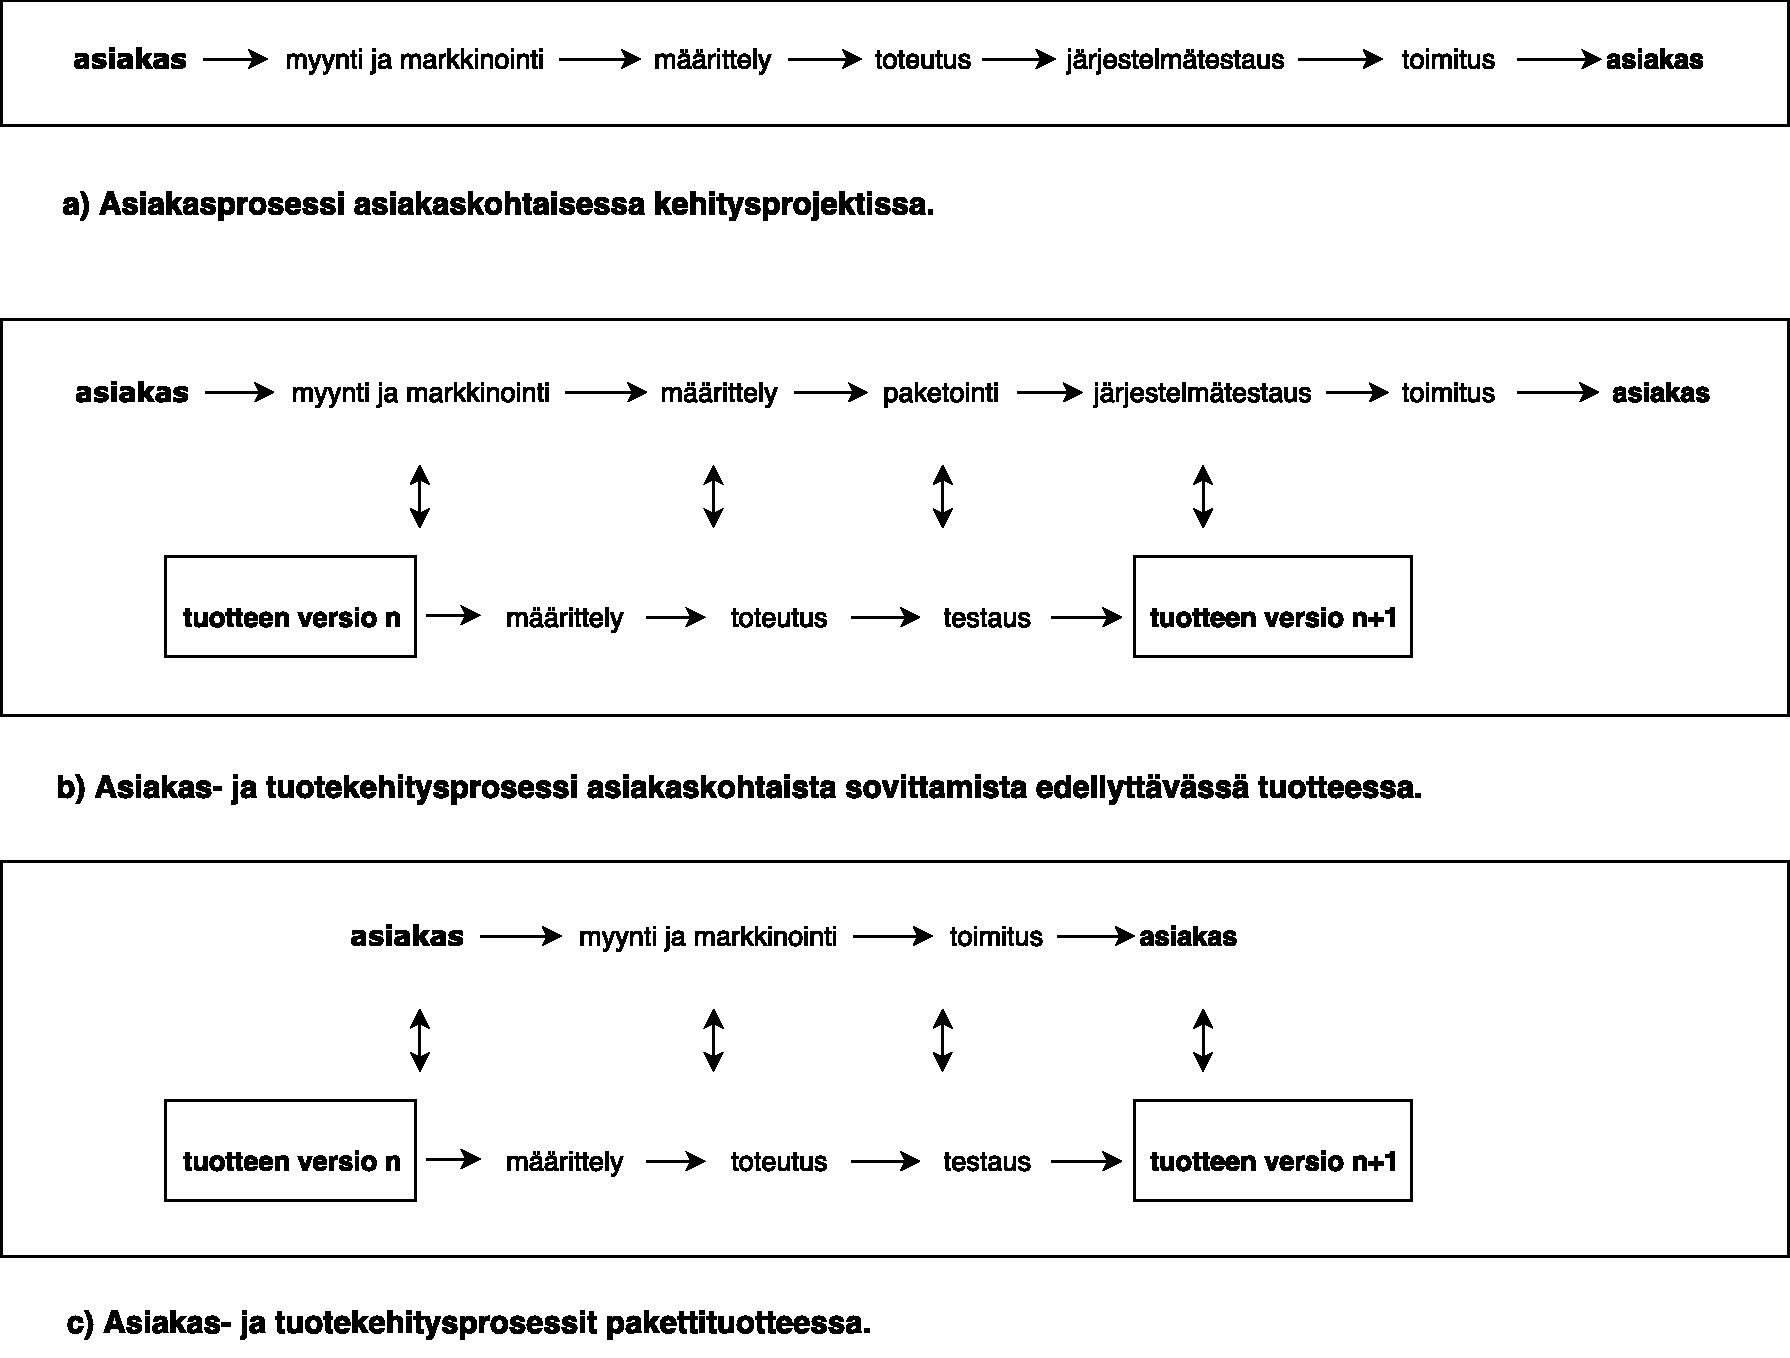
\includegraphics[scale=0.45]{asiakasprosessi.pdf}
    \caption{Asiakasprosessit eri liiketoimintamalleissa \citep{ohjelmistotuotanto}.}
    \label{fig:asiakasprosessi}
\end{figure}

Haikalan ja Marijärven mukaan on yleistä, että ohjelmistoyrityksen liiketoimintamalli sijoittuu kuvan \ref{fig:asiakasprosessi} a- ja c-liiketoimintamallien väliin. Tällöin tuotekehitys tuottaa perusmallin tuotteesta, joka paketoidaan asiakkaan toiveiden mukaan. Paketoinnilla tarkoitetaan ratkaisun kokoamista olemassa olevista komponenteista esimerkiksi konfiguroimalla. Paketointi voi myös sisältää asiakaskohtaisia muutoksia tai lisäyksiä, jolloin toiminta muuttuu asiakasprojektiksi. Yleisesti toimintaa tehostaakseen yritys pyrkii luomaan tuotteen joka on samanlainen asiakkaasta riippumatta. Usein todellisuus kuitenkin on, että asiakkaiden tarpeet vaihtelevat niin paljon, ettei asiakaskohtaiselta räätälöinniltä voi välttyä. Räätälöinnin määrää on kuitenkin hallittava, ja sen vuoksi tuotekehallinnan on oltava mukana asiakasprosessissa.

\cite{okaytannot} toteaa tuotteenhallinnan vastaavan tuotekehitysprosessista. Heidän kertovat ohjelmistotuotteiden koostuvan useista erilaisista komponenteista ja niiden erilaisista variaatioista, jotka kehittyvät tuotteen elinkaaren aikana. Ohjelmistotuotteen versio koostuu määrätystä komponenttien kokoelmasta. Tuotteenhallinta on tukitoiminto, jossa määritellään näihin asioihin liittyvät toimintatavat ja menetelmät. 

Tuotehallinta on yksinkertaisimmillaan silloin kun ohjelmistotuotteessa olevien variaatioiden määrä on pieni. Tällöin tuotteenhallinta on pääasiassa versionhallintaa, jonka tarkoituksena on helpottaa työskentelyn koordinointia tuotekehityksen aikana. Monimutkaisimmillaan tuotteenhallinta on silloin kun tuotteen konfiguraatio vaihtelee toimintaympäristöstä riippuen ja jatkokehitettävien komponenttien määrä on suuri. Jos tuotteessa on lisäksi asiakaskohtaisia sovituksia, tuotteenhallinta monimutkaistuu entisestään. \citep{okaytannot}

Asiakaskohtaista räätälöintiä vaativissa asiakasprojekteissa asiakasprosessi monimutkaistuu, koska tarvitaan erillinen määrittely-, toteutus- ja testausvaihe. Projektit vaativat myös resurssien, aikataulujen ja tehtävien määrittämistä, joita kaikkia on usein vaikea tuntea tai huomata etukäteen. Käytännössä yllättävien suunnittelemattomien tehtävien määrä voi olla jopa neljännes projektin tehtävistä sen päätyttyä. Onkin tavallista, että ohjelmistoprojektit ylittävät aikataulun ja budjetin epärealististen ennakkoarvioiden ja muuttuvien vaatimusten vuoksi. \citep{okaytannot}

Usein ongelma on historiatiedon puute vastaavista projekteista. Historiatiedon kerääminen vaatii organisaatiossa hyvin toimivaa laatujärjestelmää ja pedanttia toimintaprosessien nuodattamista, joka on usein mahdoton saavuttaa asiakaskohtaisesti muuttuvissa prosessimalleissa. Kirjoittajat esittävät, että on paradoksaalinen tosiseikka, että kaupan saa se joka on arvioinut projektin kustannukset ja valmistumispäivän eniten alakanttiin. Vaikka asiakasprojekteihin liittyykin ennalta odottamattomia asioita, ei toimintaprosessien laadusta kannata tinkiä. \citep{ohjelmistotuotanto, okaytannot}

Ohjelmistotuotteen elinkaaren kannalta suurimmat potentiaaliset säästöt ovat saavutettavissa ohjelmiston ylläpitokustannuksia pienentämällä. Tässä korostuu huolellisen suunnittelun ja ajan tasalla olevan dokumentoinnin merkitys. Usein tuotantoprosessista läpi päässeen laatuvirheen aiheuttamat kustannukset kertaantuvat ylläpitovaiheessa moninkertaiseksi. Laadunohjauksen keskeisimpiä tavoitteita onkin virheiden ennaltaehkäisy. Koska virheiden tekemiseltä ei voida kokonaan välttyä, virheet on pyrittävä poistamaan järjestelmästä mahdollisimman aikaisessa vaiheessa, jolloin kerrannaisvaikutuksilta vältytään. Näin vähenee sekä virheiden korjailun (rework) aiheuttama lisätyö kehitysprojektissa että käyttöönoton jälkeen tapahtuva ylläpitotyö. \citep{ohjelmistotuotanto}

Projektin alkuvaiheessa on vaikea tehdä rationaalisesti perusteltuja lopullisia ratkaisuja, eikä projekti voi siksi edetä alussa määritetyllä oppikirjan mukaisella prosessimallilla. Projektin alussa saadut vaatimukset muuttuvat usein projektin edetessä, ja niihin liittyvät realiteetit selviävät vasta toteutuksessa kokeilemalla. Vaikka realiteeteista olisikin hyvä käsitys alkuvaiheessa, on ihmisryhmän vaikea kollektiivisesti käsitellä niitä virheettömästi. Yksilön on helppo tarttua jo oppimaansa ratkaisuun ja siksi realiteetin vaatima toimintamalli saattaa jäädä huomaamatta. Myös jo olemassa olevien ratkaisujen uudelleenkäyttö johtaa joskus omituisiin ratkaisuihin. Näistä ongelmista huolimatta tulisi pyrkiä rationaalisen prosessimallin mahdollisimman tarkkaan seuraamiseen, koska se antaa ohjeita mitä missäkin vaiheessa pitäisi tapahtua. Tällöin projektien prosessit saadaan muistuttamaan toisiaan ja opitaan muokkaamaan niitä sopivalla tavalla tarkoituksen mukaisiksi projektin aikana, jolloin projektin suunnittelu ja seuranta on ulkopuolisenkin näkökulmasta helpompaa. Ongelmat ohjelmstotuotannossa kulminoituvat toimintaprosessin aikaisiin inhimillisiin virheisiin.\citep{ohjelmistotuotanto}

Hyvän laatujärjestelmän yksi tavoitteista onkin estää inhimilliä erehdyksiä. Inhimillisten erehdysten estäminen raskastekoisella ja monipuolisia laatustandardeja valvovalla prosessilla ei useinkaan ole paras ratkaisu. Ohjelmistojen ja järjestelmien kanssa työskentelevillä ihmisillä on usein tapana suhtautua epäilevästi kankeisiin prosesseihin, ja sen johdosta ketterät menetelmät ovat kasvattaneet suosiotaan vastareaktiona kankealle prosessille. Hyvä työprosessi ohjelmistotuotannossa onkin mahdollisimman kevyt hallittavissa oleva prosessi. Ohjelmistotuotannossa hienoinkaan prosessi ei nimittäin korvaa tekijöiden ammattitaitoa. On kuitenkin täsmennettävä, että ohjelmistotuotannon ammattilainen tehtävään soveltuvan prosessin kanssa päihittää aina toisen ammattilaisen, jolla ei ole hyvää prosessia. Ongelmaksi muodostuu juuri sopivan prosessin rakentaminen. \citep{okaytannot}

Sen vuoksi uuden prosessin rakentamista uudelleen jokaista asiakastomitusta varten tulisi välttää. Prosesseille voi toki kohdistua hyvinkin erilaisia vaatimuksia tilanteesta riippuen. Laadunhallinnan järjestelmän tulisikin tarjota valmis pohja prosessille, joka tarjoaa sopivasti taipuvan rakenteen erilaisten tavoitteiden saavuttamiseksi. Sopivan prosessin rakentaminen onkin aina kompromissi. Käytäntö on osoittanut, että prosessimallin noudattaminen ja sen toimintaan liittyvän mittatiedon kerääminen on mahdollista ja järkevää. Se mahdollistaa toiminnan kehittämisen todelliseen historiatietoon perustuen. Tämä tietysti edellyttää että toimintaprosessiton suunniteltu sillä tavalla järkeviksiettä ne ovat noudatettavissa. Amerikkalainen Victor Basili on esittänyt helpon tavan todeta tuotantoprosessin sopimattomuus: se paljastuu projektin kohdatessa ongelmatilanteen. Jos ongelmatilanteessa ensimmäiseksi unohdetaan tuotantoprosessin mukainen toiminta ja ryhdytään kiireestitekemään asioita ad hoc-tavalla niin todennäköisesti yrityksen tuotantoprosessi tulisi uusia. \citep{ohjelmistotuotanto}

Ohjelmiston kehittäminen poikkeaa muista tekniikan aloista abstraktin luonteensa takia. Ohjelmistotekniikassa on myös huomattavasti vaikeampi hahmottaa rakennettavan asian koko ja monimutkaisuus. Toinen ero ohjelmistotekniikassa konkreettisiin tekniikan aloihin on tuotantotyön ja tuotantotyöläisten puuttuminen; ohjelmistojen rakentamiseen liittyvä työ on suunnittelutyötä. Ohjelmistokehityksessä pääosissa on suunnittelu, jossa formaalilla tavalla kerrotaan tietokoneelle mitä sen pitää tehdä. Ohjelmointi sekä työkalujen käyttö ja konfigurointi on suunnittelutyötä. Formaalin suunnitelman eli ohjelman muuttamisen lopulliseksi ajettavaksi järjestelmäksi hoitaa tietokone suunnittelijan formaalien ohjeiden mukaan. Kehittämiseen liittyy olennaisena osana kehitysympäristön työkalujen, ohjelmistojen ja palvelinten valitseminen ja näiden asentaminen. Ensimmäistä kertaa tehtäessä tämä on ilman muuta suunnittelutyötä, mutta toistuessaan voi muodostua rutiiniksi. Tietotekniikassa on se mukava puoli, että kaikki rutiinit voidaan ja pitää automatisoida, niin tämäkin. Ympäristö on kuitenkin standardoitu ja tärkeimmiltä osiltaan samanlainen kaikkien kehittäjien kesken. kaikki järjestelmän asennukset kaikkiin ympäristöihin että ympäristöjen asennukset tapahtuvat automaattisesti ilman manuaalisia toimenpiteitä. Kaiken pohjana on sama suunnittelutyö, joka suurimmalta osalta on tehty jo kehitysympäristön ja ensimmäisen testiympäristön synnyttyä. Oleellista on, että myös tuotantoympäristöä koskee sama automatiikka kuin muita ympäristöjä. Järjestelmän tuotantopäivitys on yhtä kevyt operaatio kuin päivitys testiympäristöön. Tuotantoprosessin automatisointi on arkipäivää ja rakennettavissa nykypäivänä yleisesti käytössä olevilla työkaluilla. Automatisoidun tuotantoprosessin suunnittelu vaatii työtä ja osa työstä on rakennettavasta järjestelmästä riippuvaista. Aivan pienessä projektissa tuotantoprosessin täydellinen automatisointi ei välttämättä maksa itseään takaisin, mutta niissäkin tärkeimmät osat pitää ehdottomasti automatisoida. \citep{kallio}


Ohjelmistotuotannossa tavoitellaan ketterää, luotettavaa ja turvallista tuotetta. Kuitenkin käytännössä näiden kaikkien saavuttaminen on haastavaa. Usein tuotantoprosessia on vaikea määritellä ja mitata, jolloin prosessin hallitseminen on haastavaa. 

vaikeasti määriteltävissä olevat tuotantoprosessit, vaikeasti määriteltävissä ja mitattavissa olevan laatukomponentin puuttuminen, tuotanto- ja kehitysympäristön erot nostavat ylläpitokustannuksia 

Ohjelmistojen koko ja monimutkaisuus usein kasvavat liian nopeasti, jolloin menetetään tuotannon ketteryys. Tuotantoprosessia on vaikea määritellä ja siten mitata, koska ongelmat pyritään ratkomaan ketterästi. Joskus vaatimusmäärittelyssä ei osata kuvata todellista ongelmaa, joka halutaan ratkoa. 

Ohjelmistojen koko ja monimutkaisuus
Tuotantoprosessia vaikea määritellä ja siten mitata: prosessia on vaikea hallita, jos sitä ei voida mitata/ ohjelmistojen tekeminen on yhä liiaksi improvisointia/ liian vähän raakaa ja suoraviivaista työtä
Tuotteen määrittely on ongelmallista: asiakas ei oikein tiedä mitä haluaa/ määrittelyyn ei tunneta tieteellisiä, tai edes käytännössä hyvin toimivia menetelmiä
Tuotteen laadusta ei ole varmuutta: laadun formaali määrittely on vaikeaa/ ohjelmiston kattava testaus on käytännössä mahdotonta
Ohjelmistoa on työlästä pitää kunnossa: ylläpito = kaikki mikä tapahtuu ohjelman ensimmäisen käyttöönoton jälkeen/ kustannukset ovat huomattavasti suuremmat kuin kehityskustannukset

\subsubsection{Asiakasprosessin kehittäminen}

\textbf{Business process management - Prosessijohtaminen}

Business process management (BPM) is a discipline involving any combination of modeling, automation, execution, control, measurement and optimization of business activity flows, in support of enterprise goals, spanning systems, employees, customers and partners within and beyond the enterprise boundaries.

Business process management (BPM) is a discipline in operations management that uses various methods to discover, model, analyze, measure, improve, optimize, and automate business processes.[1] BPM focuses on improving corporate performance by managing business processes.[2] Any combination of methods used to manage a company's business processes is BPM.[3] Processes can be structured and repeatable or unstructured and variable. Though not required, enabling technologies are often used with BPM.[1]

As an approach, BPM sees processes as important assets of an organization that must be understood, managed, and developed to announce and deliver value-added products and services to clients or customers. This approach closely resembles other total quality management or continual improvement process methodologies and BPM proponents also claim that this approach can be supported, or enabled, through technology.[4] As such, many BPM articles and scholars frequently discuss BPM from one of two viewpoints: people

Although BPM initially focused on the automation of business processes with the use of information technology, it has since been extended[by whom?] to integrate human-driven processes in which human interaction takes place in series or parallel with the use of technology. For example, workflow management systems can assign individual steps requiring deploying human intuition or judgment to relevant humans and other tasks in a workflow to a relevant automated system.

As of 2010 technology has allowed the coupling of BPM with other methodologies, such as Six Sigma.[citation needed] Some BPM tools such as SIPOCs, process flows, RACIs, CTQs and histograms allow users to:

visualize – functions and processes
measure – determine the appropriate measure to determine success
analyze – compare the various simulations to determine an optimal improvement
improve – select and implement the improvement
control – deploy this implementation and by use of user-defined dashboards monitor the improvement in real time and feed the performance information back into the simulation model in preparation for the next improvement iteration
re-engineer – revamp the processes from scratch for better results
This brings with it the benefit of being able to simulate changes to business processes based on real-world data (not just on assumed knowledge). Also, the coupling of BPM to industry methodologies allows users to continually streamline and optimize the process to ensure that it is tuned to its market need.

\textbf{DevOps}

DevOps and its resulting technical, architectural, and cultural practices represent
a convergence of many philosophical and management movements.
While many organizations have developed these principles independently,
understanding that DevOps resulted from a broad stroke of movements, a
phenomenon described by John Willis (one of the co-authors of this book) as
the “convergence of DevOps,” shows an amazing progression of thinking and
improbable connections. There are decades of lessons learned from manufacturing,
high reliability organization, high-trust management models, and
others that have brought us to the DevOps practices we know today.
Promo - Not for distribution or sale

DevOps is the outcome of applying the most trusted principles from the
domain of physical manufacturing and leadership to the IT value stream.
DevOps relies on bodies of knowledge from Lean, Theory of Constraints,
the Toyota Production System, resilience engineering, learning organizations,
safety culture, human factors, and many others. Other valuable
contexts that DevOps draws from include high-trust management cultures,
servant leadership, and organizational change management. The result is
world-class quality, reliability, stability, and security at ever lower cost and
effort; and accelerated flow and reliability throughout the technology
value stream, including Product Management, Development, QA, IT Operations,
and Infosec.
While the foundation of DevOps can be seen as being derived from Lean, the
Theory of Constraints, and the Toyota Kata movement, many also view DevOps
as the logical continuation of the Agile software journey that began in 2001.

The principles of Flow, which accelerate the delivery of work from
Development to Operations to our customers
• The principles of Feedback, which enable us to create ever safer
systems of work
• The principles of Continual Learning and Experimentation foster
a high-trust culture and a scientific approach to organizational
improvement risk-taking as part of our daily work



Sanotaan että 95% työstä on ns waste, eliarvoa tuttamatonta

Prosessin automatisoiminen tarkoittaa, että prosessiin tuleva informaatio on ennustettavaa ja että informaation perusteella olevat lopputulokset ovat selvillä. 

On tärkeää määrittää miten paljon kannattaa asutomatisoida, koska kaiken automatisoiminen voi olla liian suuri investointi. Keskitytään tärkeimmän automatisointiin. 

Pilvipalveluistumisen myötä ohjelmistotuotanto tavoittelee liiketoimintamallissaan pääsyä mahdollisimman lähelle kuvan c-vaihtoehdon tyyppistä mallia. Se räätälöinti mitä jää jäljelle, on asiakkaan itse tekemää itsepalvelua tai käytön tukea. Tällöin resurssit voidaan kohdentaa olemassa olevian työkalujen tehokkaaseen hyödyntämiseen asiakaskohtaisen räätälöinnin sijaan. 


Key elements to identify a process for automation:

The process requires consistency across the organization
The process is repeatable
The process needs to be free from error, every time

Ohjelmistotuotannon asiakasprosessin automatisoinnissa 

Automatisoiminen tarkoittaa vaikeimpien pullonkaulojen ylitystä automaatiolla. Automaatio taas vaatii automaattisia testejä! Lempiäisen dippa.

separate man from machine. https://www.lean.org/balle/DisplayObject.cfm?o=3161 
Toimintojen jakamiseen liittyvät suunnittelupäätökset määrittävät, missä määrin annettu työ, tehtävä, toiminta tai vastuu on automatisoitu, ja missä määrin ne on annettu ihmisen suoritettavaksi... (iso..)

Tiedätkö mitä työ on? kuuntele se kohta.

Aloita manufacturing jne. 
insinöörit eri aloilta ovat hiljalleen kypsyneet tuntemaan oman työnsä sisällön. Devops handbook foreword!

Sen automatisoimisella saavutetaan three ways hyödyt. limit waste etc

Excessive automation: Rather than eliminating or at least simplifying
wasteful processes, they are often automated, creating additional
layers of system complexity and increasing total cost of ownership.




When kaizen teams perform value stream mapping, they often discover
that over 95 percent of the time, no value is added to products and services
as they move through the value stream. Information waste* is frequently
discovered to be a major cause. While some complexity is inherent to the
nature of business processes, much complexity is unnecessary and selfimposed.
We believe much of the unnecessary complexity is an outcome of
the reengineering trend of the 1990s. While significant productivity gains
were achieved during this period, the relentless pursuit of hyper-efficiency
and automation in some cases introduced overdesign and over-processing.
Aggressively pursuing automation limited flexibility and ability to change.
Over time, new products, services, and their supporting systems generated
a seemingly endless collection of intricately interwoven processes and
software, resulting in layers of non-value-adding activity. The psychological
inertia that was created remains very strong and resistant to change.
For example, during a kaizen project to improve information flow, one (Lean IT, 2010)

A holistic enterprise process viewpoint is not easily achieved, due to
the multidimensional nature of enterprise value streams and supporting
processes, shared services, projects, resources, and stakeholders.
However, if an organization is unable to identify its value streams, its
supporting processes, and their interrelationships, it will be unable to
make valid fact-based prioritization decisions on process improvements
and IT investments. 




DevOps
\subsubsection{Automaatio asiakasprosessissa}

Monilla aloilla menestyksen perusedellytyksenä on tehokkaan automaation soveltaminen. 

Automaatiolla voidaan osittain korvata työvoimaa ja pienentää tätä kautta ksutannuksia. 
uusien teknologioiden kehitys myös edesauttaa automaation yleistymistä.
perustellaan usein myös käyttöasteiden nostamisella, automaattinen jåärjestelmä tekee töitä 24/7.
Automaattisissa järjestelmissä virheiden määrä on pienempi, kuin ihmisten vastaavassa työprosessissa.
Jotkut prosessit myös vaativat tarkkuutta, joka edellyttää tietokoneohjattua käyttöä.

\cite{groover} määrittelee automaation olevan koneellinen työkalu ihmisten aikaisemmin suorittamiin tehtäviin, ja yhä enemmän tehtäviin jotka olisivat muuten mahdottomia. Tällä hän tarkoittaa koneiden integroitumista järjestelmäksi, joka kykenee toimimaan itsenäisesti ilman ihmisen väliintuloa. Hänen mukaansa automaattinen järjestelmä suorittaa prosessia sen saamien tarkkojen ohjeiden mukaisesti, ja ohjeiden noudattamista valvoo palautekontrolli, jonka tehtävä on validoida järjestelmään tulevien syötteiden oikeellisuus ja valvoa ohjeiden noudattamista prosessin aikana. 

Lähes jokaisessa yrityksessä liiketoiminta on riippuvainen tietojärjestelmistä ja niiden kehittämisestä liiketoimintavalmiuksien kasvattamiseksi. Prosessijohtamisen näkökulmasta haaste on tehdä näkyväksi tietojärjestelmiin liittyvät työprosessit. Tämä korostuu erityisesti ohjelmistotuotannon laadun johtamisessa. Perinteisessä teollisuudessa liiketoimintaprosessiin liittyvien työprosessien hallinta on viety hyvinkin pitkälle esimerkiksi Toyota Kata-filosofian edistysaskelien kautta. Liiketoimintaprosesseihin on näin pystytty rakentamaan laatu, turvallisuus ja ketteryys sisälle. 


https://devops.com/automation-versus-orchestration/ 
Se että ODI-prosessi on automaattinen tarkoittaa että se rakennetaan komponenteista joihin automaatio on rakennettu sisään. Esim. onko order-prosessi rakennettu automaatio laatukomponentti mielessä? Onko toimitusprosessi rakennettu automaatio mielessä? Onko laskutusprosessi rakennettu automaatio mielessä?
Onko meidän henkilökunta tilausten vastaanotossa 

Koska Amazonilla ei ollut logistiikkaosaamista tai olemassaolevaa rakennetta, se joutui löytämään reitin muulla tavoin, verkkokauppana jossa niitä ei tarvittu. Rakentamaan disruptiivisen ominaisuuden prosesseihinsa.

Kaikki esim 2-3-tason tyypit ovat vanhaa maailmaa, jonka läsnäolo ei auta näkemään mitä voisimme tehdä jos olisi pakko. Voisimmeko ulkoistaa toimitukset Zylincille kokonaan?

Mihin asti tuote tukee automaatiota on keskeinen kysymys?

\subsection{Asiakaspalvelujärjestelmä ohjelmistotuotteena}

Tuo esiin, että contact centerin pystytys on syytä tehdä huolellisesti koska se vaikuttaa yrityksen toimintaan isosti. Usein myös vasta käytännössä monet ongelmat selviävät.

\cite{latvakoivisto} kuvailee asiakaspalvelukeskuksen eli contact centerin olevan organisaation keskitetty toiminto, joka huolehtii asiakaspalvelusta, myynnistä ja viestinnästä asiakkaiden tai sidosryhmien kanssa. Useimmin kyseessä on kontakti digitaalisessa palvelukanavassa. Hänen mukaansa ihmisten mielikuva tästä toiminnoista on usein satojen ihmisten muodostama yksikkö, mutta Suomessa useimmat contact centerit ovat alle kymmenen hengen yksikköjä. 

\citeauthor{latvakoivisto} mukaan kontakti-sanalla viitataan viestintään asiakkaan kanssa, joka voi tapahtua missä tahansa digitaalisessa palvelukanavassa. Kontaktit erotellaan uloslähtevään ja sisääntulevaan viestintään, jolloin viestinnän välineitä on useita, ei pelkästään puheluita, vaan myös sähköposteja, yhteydenottoja Internet-sivuilta, chat-kanavasta, sosiaalisesta mediasta ja muista digitaalisista kanavista.

Asiakaspalvelujärjestelmiin liittyvät teknologiset kehitysaskeleet alkoivat automaattisen puhelinvaihteen (PABX) kehittämisestä 1960-luvulla, kertoo \cite{bernier}. Hänen mukaansa seuraava iso keksintö oli 1970-luvulla syntynyt ACD-teknologia, jonka avulla puheluita ohjataan järjestyksessä vapaalle asiakaspalvelijalle. Tämän myötä sisääntulevien puheluiden kuormaa pystyttiin hallinnoimaan ja jakamaan kuormaa tasaisesti. Samalla vuosikymmenellä nähtiin myös ensimmäiset äänivalikot puhelinvaihteissa. 1990-luvulle tultaessa tietokone yhdistyi puhelinverkkoon CTI-teknologian ansiosta, jolloin tietokoneella pystyi siirtämään tietoa puhelinverkkoon ja asiakaspalvelija pystyi käsitellä puheluita tietokoneen avulla. \citeauthor{bernier} mukaan myös Internet mullisti alaa kahdella tavalla: Kontakteja voidaan käsitellä useassa eri lokaatiossa samojen sääntöjen mukaan, ja organisaation Internet-sivut tulivat asiakaspalvelun keskiöön.

Internet ja mobiililaitteiden myötä alettiin puhua monikanavaisesta asiakaspalvelusta, sanoo \citeauthor{bernier}. Hän lisää, että tämän jälkeen yritykset havaitsivat ettei enää voi luottaa pelkkään puhekanavaan asiakaspalvelussa. Bernierin mukaan keskeistä on rakentaa yrityksen näkyvyys verkossa tavalla, joka ratkaisee useimmat asiakkaan ongelmat jo hakukoneessa. Tämän lisäksi tulisi mahdollistaa itsepalvelu verkossa mobiiliratkaisut edellä, ja mahdollistaa se, että asiakas voi hoitaa jäljelle jäävän vuorovaikutuksen yrityksen kanssa haluamassaan kanavassa. Hän tähdentää, että Internetin kautta tulevat kontaktit ovat jatkossa etusijalla vuorovaikutuksessa asiakkaiden kanssa. Asiakaspalvelua tarjoavien yritysten ja palveluntarjoajien haaste onkin pitää asiakaskokemus mielessä uusia kanavia rakentaessa, koska pelkästään uusien kanavien lisääminen ei välttämättä tehosta asiakaspalvelun toimintoja. On hyvä muistaa, että yhteyden avautuminen asiakkaan ja asiakaspalvelijan välillä on vain puolet tarinasta. Siksi asiakaspalvelujärjestelmät integroituvat yrityksen asiakashallinnan järjestelmiin. Tällöin asiakaspalvelijan on helppo saada tarvittava tieto asiakkaasta hänen ongelmansa ratkaisemiseksi.

\subsubsection{Teknologinen näkökulma} 

Tee ehkä taulukko mieluummin? ja myös ehkä eri kokoisten yritysten tarpeesta.

Perinteisiä asiakaspalvelujärjestelmän komponentteja ovat automaattinen puheluiden jakelu (ACD), tietokoneen ja puhelinliikenteen integraatio (CTI), äänivalikko (IVR), ennustava puheluiden valinta (predictive dialing), reaaliaikainen monitorointi, raportointi ja analytiikka.

Asiakaspalveluratkaisut ovat historiallisesti olleet luonteeltaan järjestelmiä, jotka on asennettu on-premises ratkaisuna yrityksen omaan konesaliin, kertovat \cite{vcc}. Tämä johtuu osittain siitä, että ne syntyivät aikana ennen Internettiä, jolloin kaikki liiketoiminnassa tarvittavat järjestelmät oli asennettava sinne missä liiketoimintaa harjoitettiin. Edelleenkin on asiakaspalvelujärjestelmä saatetaan osittain asentaa on-premises ratkaisuna esimerkiksi yrityksen omaan pilvialustaan, kertoo \cite{weiner}. Tällöin järjestelmä ja siihen liittyvä infrastruktuuri asennetaan yrityksen omaan konesaliin, ja yritys tai kumppani vastaa ylläpidosta. Etuna yrityksen näkökulmasta on kontrolli integroituihin järjestelmiin, niiden sisältämään dataan ja kustomointi omien tarpeiden mukaan. Selkeä haitta on isot investointikustannukset, ja rajoitetut mahdollisuudet integraatiolle ja tyypillisesti palvelutaso on heikompi kuin virtuaalisesti tuotetussa ohjelmistopalvelussa. 

\cite{vcc} olivat jo vuosia sitten eri mieltä. He näkivät jo silloin, että tulevaisuus on monikanavainen ja siksi on-premises asiakaspalvelujärjestelmän ei ole mahdollista tuottaa investointia takaisin. Syynä tähän oli heidän mukaansa se, että on-premises ratkaisun toimintojen kehittäminen olisi liian iso kustannus, ja investoinnit tulisi kohdentaa virtuaalisen ohjelmistopalveluna tuotetun asiakaspalvelujärjestelmän toimintojen kehittämiseen Internet-teknologioiden avulla. Virtuaalisessa asiakaspalvelujärjestelmässä yritys maksaa palveluntarjoajalle kuukausittaista tai vuosittaista maksua palvelun ylläpidosta palveluntarjoajan konesalissa. Käyttöönotto vaatii tässäkin investointia, joka on pilvi- tai selainpohjaista ratkaisua kalliimpi. Agentti käyttää järjestelmää esimerkiksi puhelinverkon tai VoIP-teknologian avulla mistä tahansa lokaatiosta. Ainoa vaatimus on verkkoyhteys ja työasema tarvittavine sovelluksineen. Tämän ratkaisun heikkous on palveluntarjoajan rajaamat  mahdollisuudet integraatiolle, kustomoinneille ja versionpäivityksille, jotka vaativat usein lisäinvestointeja \citep{talkdesk}.  

Asiakaspalvelujärjestelmiä toimitetaan myös pilvipalveluna, jolloin ratkaisu tarjotaan Internetin yli ohjelmistona tai selainpohjaisena ratkaisuna päätelaitteelle. Keskeinen hyöty pilvipalvelumallissa on multitenattisuus, jolloin käyttäjät jakavat palvelun resursseja ja ovat siten kustannustehokkaita palveluntarjoajan näkökulmasta. Tämän myötä myös palvelutaso on korkea, koska kaikki on kahdennettu. Kustannukset palvelun käyttöönotossa ja käytössä ovat huomattavasti muita pienemmät. Käyttöönottoon kuluva aika on myös minimaalinen sisältäen ainoastaan tarvittavat konfiguraatiot järjestelmään. Pilvipalveluissa hyötynä on myös se, että ne integroituvat dynaamisemmin muiden selain- ja pilvipohjaisten ratkaisujen kanssa ja ne ottavat tietoturvan, yksityisyydensuojan ja palvelutason parhaiten huomioon. Selainpohjaisissa ratkaisuissa suurin haitta on se että kaikki toiminnot tapahtuvat selaimessa, jolloin sen maailman rajoitukset ovat läsnä. \citep{talkdesk}

Virtuaalisten ja pilvipalvelupohjaisten asiakaspalveluratkaisujen myötä yhä pienemmät yritykset voivat ottaa käyttöön järjestelmän.

\subsubsection{Tulevaisuus}

Seuraavassa vaiheessa asiakkaat odottavat saumatonta vuorovaikutusta palveluntarjoajilta koska tahansa ja miten tahansa.
Asiakkaat haluavat asioida viestimällä ei soittamalla.
Chatbotit tekevät tuloaan.
Tekoälyn avulla tier 1 yhteydenotot vähenevät.

\subsection{Automaatio digitaalisessa transformaatiossa}
Kerro tässä kappaleessa miksi nyt ollaan tässä tilanteessa Telialla, että tässä yksikössä halutaan automatisoida Kontakti L:n asiakasprosessi. Miksi prosesseja pitää nyt automatisoida että voi säilyä kilpailukykyisenä? Koska DT mahdollistavat sen, ja kilpailijat yrittävät samaa
Mitkä digitaaliset teknologiat tuovat automaatiota? Esim miten multitentant tuo automaatiota, multitentant pilvip perusajatus. Relevantti koska Telia kohdentaa uusien teknologieoiden hyödyntämisen sen keskeisimpiin liiketoimintaprosesseihin.

Digitaalisten teknologioiden hyödyntäminen yrityksen liiketoimintaprosessissa alentaa liiketominnan käyttökustannuksia ja parantaa asiakaskokemusta  \citep{lamoureux, jungner}. Lamourexin mukaan yritykset, jotka omaksuvat uusien digitaalisten teknologioiden käytön liiketoiminnassaan, suoriutuvat markkinoilla kilpailijoitaan paremmin. Hän lisää, että digitaalinen transformaatio on yrityksille selviytymisen edellytys, ja kilpailukyky markkinoilla rakentuu relevanttien teknologioiden ja niiden mahdollistamien liiketoimintavalmiuksien tunnistamiseen ja rakentamiseen. 

Digitaalisuus ja siihen liittyvä automaatio ja robotiikka ovat termeinä haastavia, koska niiden merkitys jalostuu ajan kuluessa, eri ympäristössä ja yksilöiden mielissä. Ne myös kuvaavat monimutkaisia teknologisia edistysaskelia, joita on vaikea kuvata tyhjentävästi. Keskustelussa termit myös yksinkertaistuvat ja sekoittuvat toisiinsa. Onkin tärkeä muistaa, että juuri nyt niillä tarkoitetaan asioiden tekemistä aivan uudella tavalla, eikä vain automaation tai muun uuden teknologian käyttämistä nykyisissä prosesseissa. Mooren \citeyearpar{susanmoore} mukaan kyse on uuden arvon luomisesta, eikä vain parannuksista vanhaan. Hän täsmentää, että automaatio ei vähennä ihmistyön määrää, vaan ihmistyö kohdentuu luovien ratkaisujen tekemiseen teknologian avulla. Teknologia valjastetaan luomaan yksilöllistä arvoa ihmisille \citep{jungner, susanmoore}.

Digitaalisuus itsessään ei ole mikään uusi asia. Digitaalisten teknologioiden kehitys alkoi tietokoneen keksimisestä ja yleistymisestä. Internetin myötä tietokoneet ovat yhteydessä toisiinsa ja näin tieto on tarjolla paikasta ja ajasta riippumatta. Pilviteknologioiden myötä on mahdollista käyttää lähes rajaton määrä laskentatehoa ja tallennustilaa. Tietoliikenneyhteyksien kehittymisen myötä tietoa on mahdollista siirtää paikasta toiseen yhä nopeammin. Se mitä digitaalinen tarkoittaa, muuttuu edelleen kun aikaa kuluu. Tässä työssä digitaalisilla teknologioilla tarkoitetaan nimenomaan pilvestä saatavilla olevaa laskenta- ja tallennuskapasiteettia, sekä Internet-teknologioita, joiden avulla tietokoneet ovat yhteydessä toisiinsa. Tämä digitaalisuuden aalto on hyödyllinen monilla tavoin. 

Jungnerin \citeyearpar{jungner} mukaan hyötynä digitaalisuudessa on reaalimaailman asian muuttuminen tietokoneen ymmärtämään binäärimuotoon, jolloin tietokoneen laskentatehoa ja tallennustilaa voidaan käyttää todellisen maailman ilmiöiden seuraamiseen, ymmärtämiseen ja synnyttämiseen. Tällöin voidaan rakentaa työvälineitä mallintamaan reaalimaailman ilmiöitä tietokoneen maailmaan, siirtää reaalimaailman vuorovaikutusta tietokoneiden maailmaan ja avata tietokoneille tie toimia suoraan reaalimaailmassa. Teknologian kehitys mahdollistaa uusien toimintamallien syntymisen, joiden avulla yhä monimutkaisempia reaalimaailman asioita voidaan mallintaa tietokoneelle.

\subsubsection{Digitaalinen visio}

Lamourex \citeyearpar{lamoureux} kertoo, että yritys voi hyödyntää digitaalisen teknologian työvälineitä kehittääkseen tuotteita ja palveluita, tehokkaampia prosesseja ja asiakaskokemusta. Hänen mukaansa digitaalinen transformaatio tarkoittaa näiden osa-alueiden jalostumista digitaalisten teknologioiden avulla. Kaikkea ei kuitenkaan ole tarkoituksenmukaista digitalisoida kerralla, vaan jalostamisen tulisi hänen mukaansa aloittaa tunnistamalla teknologiat, joilla voidaan rakentaa liiketoimintavalmiuksia tärkeimpien pullonkaulojen ratkaisemiseen. Taulukossa \ref{tab:digkys} Lamourex esittää kysymykset, joihin digitaalisen vision antaa vastauksia.

\begin{figure}[!h]
    \centering
    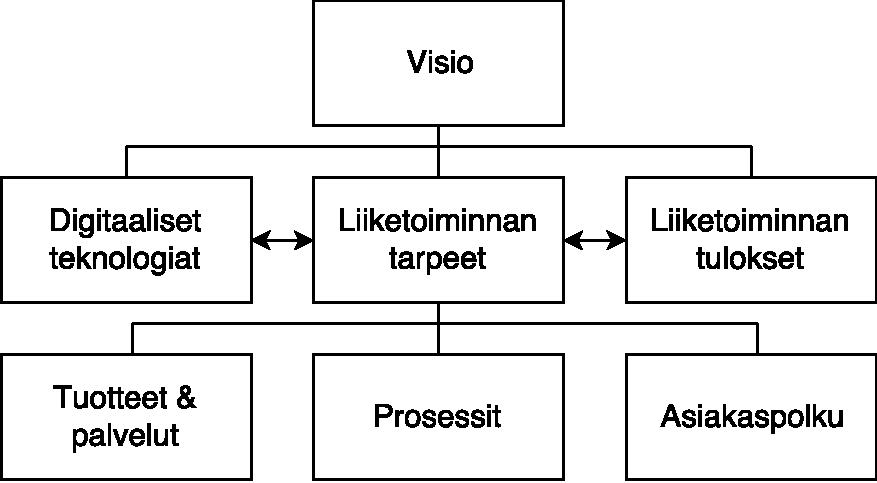
\includegraphics[scale=0.6]{images/digitaalinenvisio.pdf}
    \caption{Viitekehys digitaalisten teknologioiden hyödyntämiseen. \citep{lamoureux}}
    \label{fig:digivisio}
\end{figure}

Transformaation askeleet digitaalista visiota kohti, vaatii reaalimaailman toimintamallien arvoa tuottavan osan tunnistamista ja muuntamista tietokoneen luettavaksi, sekä arvotuotannon kehittämistä digitaalisen vision ehdoilla. Tämä vaatiikin reaalimaailmassa olevien toimintamallien pilkkomista, uudelleen järjestämistä ja eritoten karsimista \citep{leanit}. Suurin este transformaatiossa onkin organisaation vakiintunut tapa toimia, jolloin kulttuuriset näkymättömät tavat eivät sovellu digitaaliseen maailmaan \citep{jungner, lamoureux}.

MIksi transformaatio on relevantti? Sen avulla voi valjastaa digitaalisen tekemään työtä ja keskittyä luovaan asiakkaan ksilöllisseen palvelemiseen tjsp

Jungner \citeyearpar{jungner} kertoo tietokoneiden roolin korostuvan reaalimaailmassa, joka johtaa tehokkaampaan tapaan toimia. Monenlainen toiminta siirtyy tietokoneen suoritettavaksi. Tämän myötä kokonaiset toimialat uudistuvat ja myös koko yhteiskunta. Jungner käyttää esimerkkinä pankkialaa, joka käy läpi suurta muutosta, jossa palveluiden ylläpitäminen vaatii murto-osan siitä työvoimasta mitä aikaisemmin tarvittiin. Toisaalta pankkipalvelut ovat laajempia kuin aikaisemmin. Jungner alleviivaakin, että ei-digitaalisella tavalla toimiessa nykyinen pankkitoiminta vaatisi koko Suomen kansan työpanoksen. Lamourex \citeyearpar{lamoureux} korostaa, että
uusien teknologioiden hyödyntäminen ei ole vaihtoehto, vaan selviytymisen edellytys.

Jungner \citeyearpar{jungner} puhuu talouden ekosysteemin luovan tuhon kiihtymisestä nopeutuvan digitaalisuuden vuoksi, jossa vanhat yritykset, tuotteet, palvelut, tavat ja ammatit häviävät uusien tuottavampien sovellusten tieltä. Uusissa ammateissa työtavat muuttuvat hyödyntämään verkostoneituneita työvälineitä, ja tiedon hyödyntäminen tehostuu, jolloin innovaatioiden sykli nopeutuu. 

Lamourexin \citeyearpar{lamoureux} mukaan digitaalisten teknologioiden hienostuneisuus ja lukumäärä kasvaa innovaatioiden syklin nopeuduttua. Tämän myötä myös käyttötavat moninkertaistuvat. Uusien teknologioiden ja niiden käyttötapojen tehokkaalla hyödyntämisellä on mahdollista saada aikaan yhä isompia tuloksia, hän lisää. Pienet toimijat voivat vallata siivun markkinasta isommilta toimialan johtajilta tehokkaasti kohdennetulla ja ketterällä ratkaisulla. Lamourex \citeyearpar{lamoureux} puhuu disruptoinnista, jossa haastetaan vallitseva tila uudella radikaalilla tavalla, joka tuhoaa vanhaa ja luo uutta nopeasti. Hän tuo vahvasti esiin, että disruptointi ei ole vain pienten ja ketterien organisaatioiden yksinoikeus, sillä myös suuryritys voi disruptoida markkinoita. Usein suuryrityksellä onkin etulyöntiasema jos se tunnistaa nykyisten verkostojensa ja prosessiensa vahvuudet ja kykenee tekemään rohkeita kokeiluja uusien teknologioiden kanssa. 

Jungner \citeyearpar{jungner} pohtii, että puoliksi suunniteltu on digitaalisessa maailmassa tarpeeksi hyvin tehty. Hänen mukaansa käytännön kokeilut kumppaneiden ja asiakkaiden kanssa ovat nopein tapa selvittää mikä oikeasti toimii, eikä käyttää pitkää aikaa suunnitteluun. \citeauthor{devops} \citeyearpar{devops} on myös samaa mieltä: Maali liikkuu yhä nopeammin, ja siihen osuu varmemmin jos ampuu useammin ja pienemmissä erissä. Lamourex \citeyearpar{lamoureux} muistuttaa kuitenkin, että kokeiluja ohjaa digitaalinen visio uusien teknologioden tunnistaminen, joilla voi ratkaista liiketoiminnan tarpeita ja saada aikaan tuloksia. \citeauthor{gandhi} \citeyearpar{gandhi} mukaan ratkaisevaa on havaita, että digitaalinen investointi tuottaa arvoa vasta kun se on ratkaisuna tuottamassa arvoa. Kilpailussa ovat vahvoilla toimijat, jotka osaavat laittaa uudet ratkaisut työhön asiakkaiden ja muiden kumppaneiden kanssa.

\begin{table}[]
    \centering
    \begin{tabular}{l}
       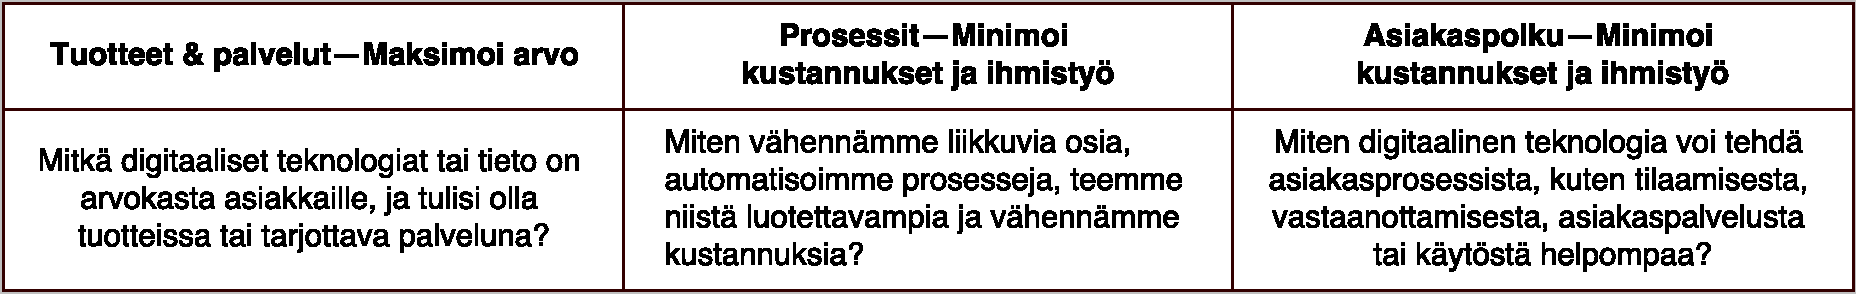
\includegraphics[scale=0.45]{images/priorisointi.pdf}
    \end{tabular}
    \caption{Kysymyksiä digitaalisen vision hahmottamiseen \citep{lamoureux}}
    \label{tab:digkys}
\end{table}

Lamourexin \citeyear{lamoureux} mukaan yrityksellä on kolme pääasiallista tapaa kehittää liiketoimintavalmiuksia markkinoilla: Kehitä tuotetta tai palvelua tekemällä siitä arvokkaampia asiakkaalle. Tehosta sisäisiä prosesseja tuottaaksesi arvo pienemmillä kustannuksilla. Paranna asiakaspolkua helpottamalla asiakkaan arvon hankkimista. Hänen mukaansa nämä osa-alueet on priorisoitava toimialan mukaan. Arvotuotannon kolme pääasiallista elementtia tuote, prosessit tai asiakaspolku korostuvat toimialan mukaan erottavana kilpailutekijänä. Investoinnit tulisi kohdentaa kilpailutekijän kehittämiseen tunnistetuille digitaalisilla teknologioilla.

Yrityksen näkökulmasta teknologialla parannetaan tuotteita, sisäisiä prosesseja ja asiakaskokemusta. Pelkästään teknologian käyttäminen ei kuitenkaan tuo hyötyä liiketoimintaan. Valitulla teknologialla täytyy olla potentiaalia kasvattaa kilpailukykyä määrätyssä aikajaksossa, ja investoinnin tulee ottaa riskit huomioon. Uusia teknologioita tulee ja menee, ja siksi tulisikin olla kykyjä tutkia useampia potentiaalisia teknologioita saman aikaisesti. Ajankohdan tulee myös olla sopiva, koska teknologiat saattavat vanhentua luultua nopeammin ja liian aikaisin tehty investointi uuteen teknologiaan saattaa heikentää kilpailuedun saamista. Teknologian hyödyntämisessä vaaditaan myös selkeä kuva liiketoimintavalmiudesta joka halutaan rakentaa sen avulla. Uusien teknologioiden käytön omaksuminen liiketoiminnan tavoitteiden saavuttamiseksi ei myöskään tapahdu itsestään. Teknologian käyttäminen kilpailuedun saavuttamiseksi markkinoilla onkin organisaation opittu taito. Eli organisaation sisäisten ja ulkoisten tavoitteen kannalta relevanttien sidosryhmien kyky tehdä yhteistyötä. Tämän kyky on vaikeampi rakentaa organisaatioissa, joissa tavoitteen kannalta relevantteja sidosryhmiä on useampia. Suurempi sidosryhmien määrä vaikeuttaa tiedon vaihtamista ja kommunikointia. Uuden teknologian hyödyntäminen kilpailiedun saavuttamiseksi vaatiikin toimintamallin muuttumista, usein yksinkertaisempaan suuntaan.

\subsubsection{Operaattorin digitaalinen transformaatio}

\subsubsection{Teknologiat digitaalisessa transformaatiossa}

Digitaalisen teknologian myötä automaatio on scriptausta apeja jne pilvessä jne. Jungner puhui kaikki on avointa



Digitalisaation työkalupakki(aoit, rpa, ...)
Digitalisaation menetelmät (devops, lean, kaikki on avointa...)
Muutosvoimat operaattorin näkökulmasta(doing digital right)
Telain strategia vastaamaan muutosvoimiin
Muutosvoimat
multi single?
Telian/operaattoreiden haasteet muutosvoimissa
- Teknologian keihäänkärjet, order to cash
Ratkaisuja tarjoavat 

teollisuudessa disruptioitiin ja sitten lähti muutos leaniin.
Automaatio ja DevOps tulee täällä. Tämän vuoksi jne.

Multi-single asiaa myös


Se että joku asia voidaan automatisoida tarkoittaa sitä että se toistuu useita kertoja samalla tavalla. Se että jokin asia toistuu useita kertoja samalla tavalla tarkoittaa, että jokin tavoitteen mukainen toiminta on onnistutaan määrämuotoistamaan toistumaan aina samalla tavalla. Jokin asia on onnistuttu määrämuotoistamaan tarkoittaa mestarillista arvoa tuottavien toimenpiteiden havaitsemista. Se
 että tunnistetaana rvoa tuottavat toimenpiteet tarkoittaa työprosessien hyvää tuntemusta siitä mitä arvoa tuottava työ on. se että tuntee mitä arvoa tuottava työ on tarkoittaa oman työn ja itse arvon tuntemista.
arvon tuntemista
streamlinattu toistamaan asioita jotka auttavat pääsemään tavoitteeseen. 


\subsection{Kappaleen yhteenveto}


Ydinprosessit Telialla ja ODI prosessi niiden joukossa. Minkälaista tehtävää se suorittaa?

\clearpage

\section{Tutkimusaineisto ja -menetelmät}
%\section{Materials and methods}
\subsection{Tutkimusmotiivi}
\subsection{Tutkimusmenetelmä}
\subsection{Case Telia Kontakti L}
\subsubsection{New Generation Telco}
\subsubsection{CC-ratkaisut - Zylinc}
\subsubsection{CC-markkina}
MUOKKAA: https://jyx.jyu.fi/dspace/bitstream/handle/123456789/47339/URN%3aNBN%3afi%3ajyu-201510203424.pdf?sequence=1 


Tukitaan elementtejä joiden välille automaatio on rakennettava, keskeinen on miten itse tuote tukee automaatiota. Sen jälkeen mietitään mihin asti voidaan tehdä perusmalli, ja katsotaan miten paljon konfiguraatiota jää jäljelle. Sitten katsotaan miten organisaation tarjoamat työkalut tilauspäähän tukevat jäljelle jäävän konfiguraation tekemistä itse. Pilvipalvelut integroituvat dynaamisemmin toisiinsa. Tunnista ns legacyt ja front endit.


https://aaltodoc.aalto.fi/bitstream/handle/123456789/20153/master_Honkanen_Heikki_2016.pdf?sequence=1 

Saaranen-Kauppisen ja Puusniekan (2006) mukaan laadullinen tutkimus soveltuu hyvin pääosin elämismaailman merkitysten tutkimiseen, ja siinä tutkimusaineisto on kooltaan suhteellisen pieni. Tutkimus rakentuu yleensä aiemmista alan tutkimuksista, empiirisestä aineistosta sekä tutkijan omasta päättelystä. Laadullisessa tutkimuksessa ei ole ennakkohypoteeseja, joita pyritään todentamaan, vaan tutkimuksen tarkoitus on pikemminkin keksiä hypoteeseja. (Saaranen-Kauppinen & Puusniekka, 2006). 

Tapaustutkimus valittiin tutkimusmenetelmäksi, koska se soveltuu Järvisen ja Järvisen (2012) mukaan hyvin aiheiden kuvaamiseen, joita ei ole tutkittu paljoa aiemmin. Tapaustutkimuksessa käsitellään yksittäistä, rajattua kokonaisuutta luonnollisessa ympäristössään, ja kuvaillaan tutkimuskohteen ominaispiirteitä tarkasti ja totuudenmukaisesti (Saaranen-Kauppinen & Puusniekka, 2006). 

Nomovok valittiin tapaustutkimuksen kohteeksi, koska se muodostaa tapauksena hyvän esimerkkikokonaisuuden aihepiiristä. Yritys on vakiintunut toimialallaan, sen
liiketoimintamalli on muuttunut hiljattain ja sen liiketoimintamallia pystytään tarkastelemaan muutoksen näkökulmasta eri ajanhetkillä. Lisäksi suuri osa ohjelmistoyritysten liiketoimintamalleja käsittelevästä tutkimuksesta liittyy eliiketoimintaan, ja tämä tutkimus haluttiin toteuttaa perinteisemmän ohjelmistoliiketoiminnan näkökulmasta, jollaista Nomovok harjoittaa.

Tapaustutkimuksessa aineistoa tulisi kerätä monenlaisista lähteistä, koska esimerkiksi yksittäinen haastattelu voi antaa vääränlaista tietoa ja koska useita lähteitä yhdistelemällä pystytään arvioimaan kerätyn tiedon oikeellisuutta ja olennaisuutta (Järvinen & Järvinen, 2012). Aineistonkeruu tähän tapaustutkimukseen suoritettiin haastattelemalla yrityksen johtoa ja tutustumalla olemassaolevaan kirjalliseen markkinointimateriaaliin.

Haastattelu valittiin aineistonkeruumenetelmäksi, koska SaaranenKauppisen
ja Puusniekan (2006) se soveltuu hyvin, jos tutkimusaiheena on laaja
kokonaisuus, jota ei ole kyseisessä ympäristössä tutkittu aiemmin, ja josta
halutaan mahdollisimman analyyttista. Lisäksi ei haluttu suoraan olettaa, että
tapausyrityksen liiketoimintamalli vastaa elementeiltään
kirjallisuuskatsauksessa luotua kehikkoa, ja haastattelun avulla oli helppoa
selvittää yrityksen edustajien näkemys asiasta. Haastattelut olivat
puolistrukturoituja, jolloin kerättävä tieto oli mahdollisimman analyyttista ja
kattaa mahdollisimman laajasti aihepiirin, mutta sisältö pysyy silti aihepiirin
rajoissa (Järvinen & Järvinen, 2012). Puolistrukturoidussa haastattelussa
esitetään samat kysymykset kaikille haastateltaville, mutta ei välttämättä
samassa järjestyksessä, ja lisäksi kysmykset on pidetty korkealla tasolla, jotta
vastaajalla on liikkumavaraa aiheen sisällä (Saaranen-Kauppinen & Puusniekka,
2006). 

Case study: yksilöllinen tapaus

Tapaustutkimus on paljon käytetty menetelmä liiketaloustieteen piirissä tutkittaessa yrityksiä ja organisaatiokäyttäytymistä.

Tutkittavat tapaukset ovat ainutkertaisia, ja niitä tutkitaan omassa erityisessä ympäristössään.

Tärkeää on tutkimusasetelman kytkeytyminen aikasempaan teoriapohjaan, joka muodostaa perustan jolta analyysit ja tulkinnat tehdään johtopäätelmissä.
Tutkija ja tutkimuskohde ovat case-tutkimuksessa läheisessä vuorovaikutuksessa keskenään, ja luottamuksen säilyttäminen on osa tutkimusprosessia. Tuloksissa pyritään ymmärtämään ja tulkitsemaan syvällisesti yksittäisiä tapauksia niiden erityisessä kontekstissa, haetaan tietoa dynamiikasta ja prosesseista.

Tieto kerätään haastatteluilla, koska prosessit ovat suurimmaksi osaksi tuotepäälliköiden korvien välissä tai yksittäisissä dokumenteissa.

Prosessiinfrastructuuri on olemassa, mutta sen yhteys toimintamalleihin on vielä heikko. 

Tuotteistusprojekti joka vastaa ODI-prosessin luomisesta on projekti, jonka tuloksena automatisoitu ODI-prosessin tulisi syntyä. Joten siksi onkin syytä tarkastella miten tuotteistusprojekti toimii.


ODI-prosessi koostuu osaprosesseista ja niiden komponenteista. Mihin laatuvaatimuksiin nykyiset komponentit ovat rakennettu?



MIssä liiketominta casessa automaatiota tulisi hyödyntää. 

Tutki miten ODI-prosessi rakennetaan Telialla juuri nyt.

Tutki valmiita komponentteja ja kun niitä yhdistellään tutki mahdollisia manuaalisia työvaiheita jotka ovat riski.

Koko business case asiaakspalvelujärjestelmätoimituksissa.

Tässä osassa kuvataan käytetty tutkimusaineisto ja
tutkimuksen metodologiset valinnat, sekä
kerrotaan tutkimuksen toteutustapa ja käytetyt menetelmät. 

\clearpage

\section{Havainnot}
%\section{Results}

Myynti toivoo kuumeisesti toimintoja tuotteisiin, että he voivat myydä niitä ja esitellä niitä asiakkaille.

Miten ODI-prosessi rakennetaan Telialla???
Nykyinen laatujärjestelmä ODI-prosessin tekemiseen ei ole määritelty, vaan tuotepäälliköiden päässä.
Laatujärjestelmä on ODi-labraus. Miten se vastaa laatumittauksesta?

Olosuhteet ovat sellaiset joissa voidaan pilkkoa koko arvotuotanto pieniin osiin, jolloin voidaan ydin arvo tuottaa pienissä mutta nopeissa erissä. ALoitetaan ydinjutusta ja laajennetaan sitä samalla kun tietämys ja mestarillisuus pienistä ydin osista alkaa kasaantua. Toisto luo oppia ja oppi mestarillisuutta. Silloin voidaan nähdä 

MUltitenant on tärkein pilviteknologioiden lähtökohtahttp://www.zdnet.com/article/defining-the-true-meaning-of-cloud/?tag=mantle_skin;content
Tämän jälkeen yhteydet joko sdwan tai internet, ei datanettiä.

Pitää osata tuotteistaa jotain sellaista joka vastaa asiakastarvetta ja kun siitä saadaan kokemusta lyhenee läpimeno ja opitaan mestareiksi tehostamisessa. Tämän jälkeen voidaan sanoa mitä kannattaa automatisoida. Siihen robotisaatiomalliin on saatava vihreät valot. Eli on osattava vastata kysymyksiin tarkasti!

Miksi pilotoitiin mehiläisen kanssa joka ei vastaa ollenkaan sitä mihin koko0 zylincci hankittiin? Pinillä incrementeillä?

Tässä osassa esitetään tulokset ja vastataan tutkielman alussa
esitettyihin tutkimuskysymyksiin. Tieteellisen kirjoitelman
arvo mitataan tässä osassa esitettyjen tulosten perusteella. 

%% Huomaa seuraavassa kappaleessa lainausmerkkien ulkopuolella piste, 
%% koska piste ei lopeta lainattua tekstinpätkää.
%% Jos lainattu tekstinpätkä loppuu välimerkkiin, tulee välimerkki
%% lainausmerkkien sisälle: 
%% "Et tu, Brute?" sanoi Caesar kuollessaan.
Tutkimustuloksien merkitystä on aina syytä arvioida ja tarkastella
kriittisesti.  Joskus tarkastelu voi olla tässä osassa, mutta se
voidaan myös jättää viimeiseen osaan, jolloin viimeisen osan nimeksi
tulee >>Tarkastelu>>. Tutkimustulosten merkitystä voi arvioida myös
>>Johtopäätökset>>-otsikon alla viimeisessä osassa. 

Tässä osassa on syytä myös arvioida tutkimustulosten luotettavuutta.
Jos tutkimustulosten merkitystä arvioidaan >>Tarkastelu>>-osassa,
voi luotettavuuden arviointi olla myös siellä. 

\clearpage

\section{Tutkimuskysymyksiin vastaaminen}

\section{Yhteenveto}
%\section{Summary} 

Opinnäytteen tekijä vastaa siitä, että opinnäyte on tässä dokumentissa
ja opinnäytteen tekemistä käsittelevillä luennoilla sekä
harjoituksissa annettujen ohjeiden mukainen muotoseikoiltaan,
rakenteeltaan ja ulkoasultaan.



\clearpage
%% Lähdeluettelo
%%
%% \phantomsection varmistaa, että hyperref-paketti latoo hypertekstilinkit
%% oikein.
%%
%% The \phantomsection command is nessesary for hyperref to jump to the 
%% correct page, in other words it puts a hyper marker on the page.

\phantomsection
%\addcontentsline{toc}{section}{Viitteet}
%\addcontentsline{toc}{section}{References}
%%\begin{thebibliography}{99}
\bibliography{lahteet}

%% Alla pilkun jälkeen on pakotettu oikea väli \<välilyönti>-merkeillä.

%%\end{thebibliography}

%% Liitteet 
\appendix 
\clearpage
%% Lisää tekstin "Liitteet" sisällysluetteloon
%%
%% Adds the word "Appendices" to the table of contents
\addtocontents{toc}{\protect\contentsline{section}{Liiteet}{}{appendix}}
%\addtocontents{toc}{\protect\contentsline{section}{Appendices}{}{appendix}}

\section{Esimerkki liitteestä\label{LiiteA}}
%% Liitteiden kaavat, taulukot ja kuvat numeroidaan omana kokonaisuutenaan
%%
%% Equations, tables and figures have their own numbering in Appendices
\renewcommand{\theequation}{A\arabic{equation}}
\setcounter{equation}{0}  
\renewcommand{\thefigure}{A\arabic{figure}}
\setcounter{figure}{0}
\renewcommand{\thetable}{A\arabic{table}}
\setcounter{table}{0}

Liitteet eivät ole opinnäytteen kannalta välttämättömiä ja 
opinnäytteen tekijän on 
kirjoittamaan ryhtyessään hyvä ajatella pärjäävänsä ilman liitteitä.
Kokemattomat kirjoittajat, jotka ovat huolissaan
tekstiosan pituudesta, paisuttavat turhan 
helposti liitteitä pitääkseen tekstiosan pituuden annetuissa rajoissa.
Tällä tavalla ei synny hyvää opinnäytettä.   

Liite on itsenäinen kokonaisuus, vaikka se täydentääkin tekstiosaa.
Liite ei siten ole pelkkä listaus, kuva tai taulukko, vaan 
liitteessä selitetään aina sisällön laatu ja tarkoitus. 

Liitteeseen voi laittaa esimerkiksi listauksia. Alla on 
listausesimerkki tämän liitteen luomisesta. 

%% Verbatim-ympäristö ei muotoile tai tavuta tekstiä. Fontti on monospace.
%% Verbatim-ympäristön sisällä annettuja komentoja ei LaTeX käsittele. 
%% Vasta \end{verbatim}-komennon jälkeen jatketaan käsittelyä.
\begin{verbatim}
	\clearpage
	\appendix
	\addcontentsline{toc}{section}{Liite A}
	\section*{Liite A}
	...
	\thispagestyle{empty}
	...
	tekstiä
	...
	\clearpage
\end{verbatim}

Kaavojen numerointi muodostaa liitteissä oman kokonaisuutensa:
\begin{eqnarray}
d \wedge A  &=& F, \label{liitekaava1}\\
d \wedge F  &=& 0. \label{liitekaava2}
\end{eqnarray}


\clearpage
\section{Toinen esimerkki liitteestä\label{LiiteB}}

%% Liitteiden kaavat, taulukot ja kuvat numeroidaan omana kokonaisuutenaan
%%
%% Equations, tables and figures have their own numbering in Appendices
\renewcommand{\theequation}{B\arabic{equation}}
\setcounter{equation}{0}  
\renewcommand{\thefigure}{B\arabic{figure}}
\setcounter{figure}{0}
\renewcommand{\thetable}{B\arabic{table}}
\setcounter{table}{0}

Liitteissä voi myös olla kuvia, jotka
eivät sovi leipätekstin joukkoon:
%% Ympäristön figure parametrit htb pakottavat
%% kuvan tähän, eikä LaTeX yritä siirrellä niitä
%% hyväksi katsomaansa paikkaan. 
%% Ympäristöä center voi käyttää \centering-
%% komennon sijaan
%%
%% Example of a figure, note the use of htb parameters which force
%% the figure to be inserted here
\begin{figure}[htb]
\begin{center}
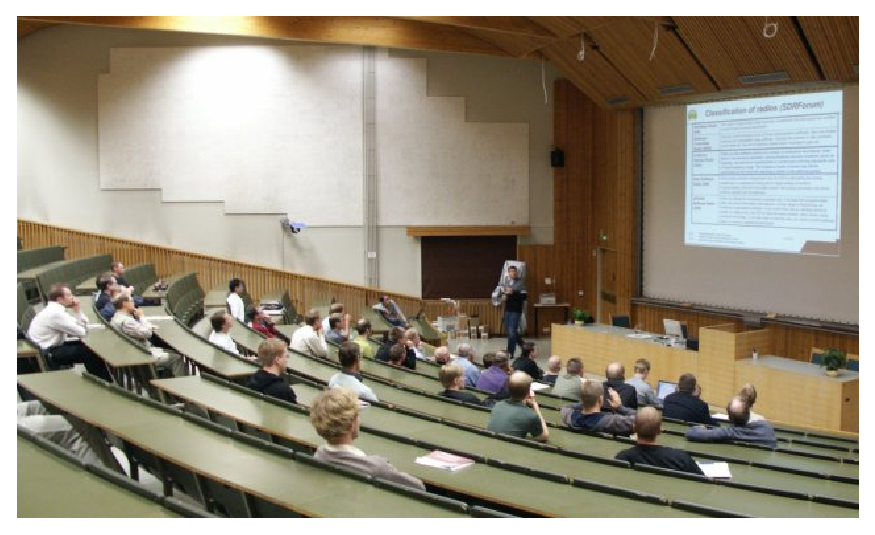
\includegraphics[height=8cm]{kuva2}
\end{center}
\caption{Kuvateksti, jossa on liitteen numerointi \label{liitekuva}}
\end{figure}
%%
Liitteiden taulukoiden numerointi on kuvien ja kaavojen kaltainen:
\begin{table}[htb]
\caption{Taulukon kuvateksti. \label{liitetaulukko}}
\begin{center}
\fbox{
\begin{tabular}{lp{0.5\linewidth}}
9.00--9.55  & Käytettävyystestauksen tiedotustilaisuus (osanottajat
ovat saaneet sähköpostitse valmistautumistehtävät, joten tiedotustilaisuus
voidaan pitää lyhyenä).\\
9.55--10.00 & Testausalueelle siirtyminen
\end{tabular}}
\end{center}
\end{table}
Kaavojen numerointi muodostaa liitteissä oman kokonaisuutensa:
\begin{eqnarray}
T_{ik} &=& -p g_{ik} + w u_i u_k + \tau_{ik},  \label{liitekaava3} \\
n_i    &=& n u_i + v_i.                        \label{liitekaava4}
\end{eqnarray}

\end{document}
